% A sample model to write a thesis project

% Search for the string "TBC: " and follow the instructions

\documentclass[titlepage,openright,twoside,a4paper,final,12pt]{book}

%%% TBC: Select your language here: english or spanish
\usepackage[spanish]{babel}
\usepackage[utf8]{inputenc}
\usepackage[pdftex,final]{graphicx}

% Style package
\usepackage{trinidad-PhD}
% Font Package (Palatino)
\usepackage{mathpazo}
% Packages for specific capabilities
\usepackage{rotating} % for text rotation in tables
\usepackage{multirow} % for multirow in tables
\usepackage{subfigure} % Place subfigures in figure environment
% Packages for specific symbols
\usepackage{amssymb}
\usepackage{amsmath}
\usepackage{amsfonts}
\usepackage{eurosym} % Euro symbol
\usepackage{bbding} % for \XSolidBrush
\usepackage{pifont} % for \ding{55} (a check mark)
\usepackage{fancyvrb,fancybox,calc}
\usepackage{soul}
\usepackage{multirow}
%\usepackage[xindy]{imakeidx}
%\makeindex

\usepackage[style=numeric-comp,backend=bibtex]{biblatex}
\bibliography{refs.bib}

\author{Sergio Rodríguez Calvo}{D.~}{XXXXXXXXL}
\authorURL{}
\authorEMail{sergiorodriguezcalvo@gmail.com}
\setTitle{Análisis de las transiciones de comportamiento en crecimiento de tumores usando una simulación con autómata celular}
\setSubtitle{}
\setUniversity{Universidad de Sevilla}
%\supportText{Memoria para el trabajo fin de máster}
%\copyrightText{}
\committeeMember{}
\committeeMember{}
\committeeMember{}
\committeeMember{}
\supervisor{Miguel Ángel Gutiérrez Naranjo}{Dr.~}{Profesor Titular del Departamento de Ciencias de la Computación e Inteligencia Artificial de la Universidad de Sevilla}

\begin{document}
	\makeTitlePage

	\pagestyle{empty}
	\pagenumbering{arabic}
	\pagestyle{trinidadPhD}

	\tableofcontents
	\listoffigures

    \chapter{Resumen}
		El cáncer es un nombre genérico que agrupa más de 200 enfermedades\footnote{\url{https://www.aacrfoundation.org/Pages/what-is-cancer.aspx}}
que causan proliferación descontrolada de células provocando la aparición de masas anormales. A toda masa anormal se
le conoce como neoplasia y, según su invasividad y factor de crecimiento, puede ser maligna (carcinoma) o benigna (adenoma).

Esta enfermedad puede ser vista como un comportamiento emergente, que puede ser explicado a
partir de la presencia de ciertos marcadores cancerosos a nivel local.

José Santos y Ángel Monteagudo, autores de una serie de artículos \cite{jsantos-amonteagudo-2012} \cite{jsantos-amonteagudo-2013} \cite{jsantos-amonteagudo-2015} y, entre ellos, el artículo
en el que se centra este trabajo \cite{jsantos-amonteagudo-1-2014}, proponen el uso de autómatas
celulares como técnica para simular dicho comportamiento dada su idoneidad.

Se propone una modelización en la cual se utiliza una rejilla en tres dimensiones donde, sin
tener en cuenta el tamaño de la célula, se presenta al comienzo una única célula en el centro de dicha
rejilla. Cada célula, cuenta con un genoma asociado que representa la aparición de mutaciones,
así como, dos propiedades: tamaño del telómero, y tasa de mutación base.

Todo ello, es utilizado dentro de un modelo de eventos, en el cual, se programan eventos mitóticos
en el futuro y en el que se consideran una serie de pruebas previas a la mitosis. Dichas pruebas,
modelizan el comportamiento individual de cada célula a la hora de ejecutar la división, así como,
todos aquellos factores que pueden derivar en la muerte de la célula y factores provocados
por las mutaciones adquiridas.

Finalmente, se realizan una serie de simulaciones, alterando los parámetros de configuración del
autómata, con el objetivo de estudiar el nuevo comportamiento, así como, la incidencia
de determinadas terapias en el comportamiento global del sistema.


		\chapter{Introducción}
		Desde el punto de vista de la biología computacional el cáncer puede ser visto como un sistema ecológico y de comportamiento emergente.
Lo cual, hace apropiado el uso de autómatas celulares para simular su comportamiento. Es por ello que, cada vez más se opta por el uso
de simulaciones por ordenador como la que se presenta en este trabajo ayudando, desde el estudio y comprensión del cáncer, hasta
el estudio y desarrollo de nuevas terapias contra él.

El cáncer es una enfermedad cada vez más común debido a sus muy diversos factores que propician su aparición, esto es,
mayor esperanza de vida de la población y, por tanto, individuos cuyas células han sufrido más mutaciones, factores ambientales y/o
formas de vida poco saludables, mayor estrés de la población, y hasta exposición a fuentes de radiación artificiales.

A pesar de todo, el cuerpo tiene una serie de mecanismos para prevenir la aparición y la proliferación de esta enfermedad. Estos,
son muchos y muy diversos, así como, los mecanismos propios de las células que intervienen en este proceso. En esta simulación, por tanto,
se pretende tener en cuenta el enfoque de los autores del trabajo original, eligiendo sólo un subconjunto de todas estas
carácteristicas y comportamientos.

La elección de un autómata celular como enfoque para modelizar el comportamiento de esta enfermedad proviene por la relativa
facilidad de obtener comportamientos complejos a partir de una reglas relativamente sencillas a nivel local en cada célula.

Este trabajo, como se ha comentado previamente, pretende reproducir el trabajo de José Santos y Ángel Monteagudo \cite{jsantos-amonteagudo-1-2014},
uno de los trabajos \cite{jsantos-amonteagudo-2012} \cite{jsantos-amonteagudo-2013} \cite{jsantos-amonteagudo-2015} que dichos autores han realizado siguiendo la idea de realizar simulaciones sobre esta enfermedad y, por ello, aquí
se realiza una nueva implementación con el fin de reproducir los resultados obtenidos en el citado artículo.

\newpage

La implementación consiste en seguir un modelo de eventos, es decir, se pretende simular el proceso que siguen las células para su división, que
consiste en, la realización de una serie de pruebas para comprobar si la célula debe reproducirse, la realización de la propia división, y
la programación de un nuevo evento de división en el futuro. A lo largo de la ejecución del programa en cada iteración puede haber ninguna, una o
varias células que deben seguir el proceso que se acaba de describir brevemente.

Finalmente, para estudiar el comportamiento del cáncer se realizan diversas ejecuciones utilizando diferentes parámetros y configuraciones,
y observando en cada caso qué factor es el que provoca el cambio en el comportamiento global.

\section{Objetivos}

En este trabajo, se esperan alcanzar los siguientes objetivos:

\begin{itemize}
  \item Encontrar artículos científicos de calidad sobre esta temática.
  \item Extraer información del artículo (o los artículos).
  \item Elegir un artículo y hacer una implementación propia.
  \item Reproducir los resultados del artículo.
  \item Comparar los resultados obtenidos con los del artículo.
\end{itemize}

\section{Alcance}

El presente trabajo tiene como finalidad reproducir el trabajo de José Santos y Ángel Monteagudo \cite{jsantos-amonteagudo-1-2014}, realizando
una implementación propia del sistema que se describe en su artículo.

No obstante, el comportamiento que se pretende simular cuenta con una serie de pasos en los cuales el comportamiento dependerá
de ciertos sorteos con una probabilidad dada. Esta es una limitación a tener en cuenta a la hora de obtener los mismos resultados
que los autores de dicho trabajo.

\section{El cáncer}

El cáncer es el nombre genérico usado para referirse a más de $200$ enfermedades cuyo resultado
es la proliferación descontrolada de las células que se ven afectadas. Aunque no era común
encontrar signos de cáncer en los seres vivos en la antigüedad debido a una menor esperanza
media de vida, lo cierto es que es inherente al reino animal.

El origen etimológico del nombre proviene de la antigua grecia, donde
Hipócrates utilizó los términos \textit{carcino} y \textit{carcinoma} para referirse
a dicha enfermedad, las cuales hacían referencia al cangrejo debido a la forma en la
que se proyectaban los cánceres.

El cáncer se clasifica como:

\begin{itemize}
    \item Una \textbf{enfermedad genética}, debido a, que es causada por un cambio en el
    material genético (\textit{ADN}) de las células.
    \item Una \textbf{enfermedad multigénica}, ya que, afecta a diferentes genes.
    \item Una \textbf{enfermedad multifactorial}, es decir, tiene causas muy diversas.
    \item Una \textbf{enfermedad multiorgánica}, por tanto, afecta a diferentes tejidos y órganos.
\end{itemize}

Se conoce como neoplasia a toda masa anormal que tenga lugar en el cuerpo. Esto es, la división
descontrolada de la célula y el aumento de tamaño de cada una de ellas, y ocurre
por un problema en el \textit{ADN} de la célula, la cual, contiene la información acerca de cuales son
las funciones de la misma.

Al producirse en todo tipo de tejidos la evolución y el tratamiento de esta enfermedad varía.
El factor determinante entre que este tipo de masas anormales sea benigna (adenoma)
o maligna (carcinoma) es el factor de crecimiento y la invasividad de tejido adyacente.

Presenta diferentes fases, partiendo de un crecimiento anormal en tamaño, en la cual,
las células del interior necesitarán más sangre para obtener nutrientes y, en consecuencia,
mueren por necrosis. El tumor puede pasar a una nueva fase, conocida como \textit{angiogénesis},
si adquiere la capacidad de crear nuevos vasos sanguíneos para alimentar a las células
del interior. Esto lo consigue mediante el envío de señales químicas que motiva la creación
de nuevos capilares hacia dentro del tumor, generando nuevos vasos sanguíneos a partir de
los preexistentes. Finalmente, la célula se vasculariza, es decir, partes de ella pasan
a la sangre, continuando con este comportamiento allí donde se depositen y, además, en muchas
ocasiones se observa metástasis.

Es obvio, que la célula para llegar a la última fase va a necesitar cierto grado de daño genético,
así como, superar determinadas barreras. Por un lado, obtener todas las capacidades necesarias para
poder dividirse sin control, crear sus propios vasos sanguíneos, etc. dependerá de la obtención
de mutaciones en su \textit{ADN} que permita todo esto. Por otro lado, el cuerpo tiene mecanismos para evitar
que esto ocurra, como por ejemplo, muerte por daño genético, evitar enviar orden de división e, incluso,
el propio sistema inmune interviene para intentar evitar su crecimiento, además de otros muchos mecanismos.

Por tanto, esta es una enfermedad compleja de tipo ecológico y emergente, lo cual, dificulta su estudio,
así como, su tratamiento.

\section{Los autómatas celulares}

El patrón mostrado en ciertas conchas marinas, como se muestra en la figura ~\ref{fig:conus},
es generado mediante autómatas celulares naturales. Estas conchas muestran un aspecto exterior
en el cual se observan patrones, los cuales les han
permitido en muchas ocasiones ocultarse mejor en su entorno y, por ello, aumentar su supervivencia.
Dichos patrones son de muy diversos tipos, por ejemplo, forman formas reconocibles, o formas fractales,
entre otras.

\begin{figure}[h]
\centering
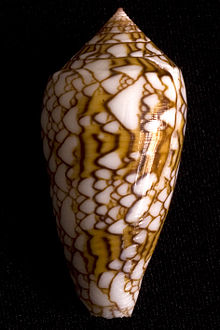
\includegraphics[scale=2]{figures/Conustextile}
\caption{\textit{Conus textile shell}, especie de gasterópodo que presenta un autómata celular natural en su concha.}
\label{fig:conus}
\end{figure}

\newpage

En ellos, cada célula toma un color o forma diferente según sus células vecinas, obedeciendo
a una versión natural de unas reglas matemáticas. Basándose en esto, se conoce como autómata celular
al modelo matemático abstracto que modela sistemas dinámicos que evolucionan en pasos discretos.

Son muy adecuados para ser implementados por ordenadores, útiles para simular comportamientos de sistemas
complejos, como por ejemplo: colonias, epidemias, dinámica de fluidos, etc., y en muy diversas áreas, como por ejemplo,
en física, biología, química, socioeconomía, etc.

En el libro \textit{Simulating Complex Systems by Cellular Automata} de Jiri Kroc, Peter M.A. Sloot y Alfons G. Hoekstra
\cite{cellular-automata} se presentan los fundamentos matemáticos que siguen los autómatas celulares.

Fueron descubiertos por John von Neumann en la década de 1950, aunque basado en trabajos teóricos previos de la
década de 1940. A modo de resumen, los autómatas celulares cuentan con los siguientes componentes:

\begin{itemize}
    \item Red regular de nodos, de cantidad finita o infinita, que representa la estructura espacial.
    \item En cada nodo, se coloca un autómata finito, es decir, representa un número finito de estados posibles.
    Aquellos que se encuentran ocupados, reciben el nombre de células o celdas.
    \item Cada célula se comunica con su entorno, pero sólo con una parte de él. Esto se conoce como vecindario,
    y existen varios tipos, por ejemplo, el vecindario de Moore, o el vecindario de vonNeumann,
    como se muestra en la figura ~\ref{fig:neighboor}.
    \item Función que determina la evolución de los estados de las distintas células.
\end{itemize}

\begin{figure}[h]
\centering
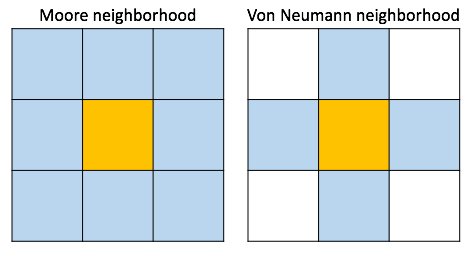
\includegraphics[scale=0.6]{figures/automata_neighboor}
\caption{Tipos de vecindarios en los autómatas celulares.}
\label{fig:neighboor}
\end{figure}

Dada una configuración se puede estudiar las transformaciones aplicando las reglas,
lo que se conoce como órbita. Dichas órbitas pueden ser muy complejas, a pesar de
la sencillez del autómata celular.

Uno de los autómatas celulares más famosos es el \textit{Juego de la vida de Conway}.
Diseñado por el matemático John Horton Conway en la década de $1970$. Es tan famoso debido a
que es equivalente a una máquina universal de Turing o, lo que es lo mismo, es un modelo de computación universal\footnote{\url{http://eprints.uwe.ac.uk/22323/1/thesis.pdf}}.
Esto es, todo lo que se puede computar algorítmicamente se puede computar en el juego de la vida.

Existen, además, muy diversas implementaciones y aplicaciones, como por ejemplo, para hacer música.
En el libro \textit{Game of Life Cellular Automata} de Andrew Adamatzky \cite{game-of-life} se presenta
el juego de la vida, y en el último capítulo se expone una forma de hacer música con él. Para ello, el autor
utiliza cada celda ocupada por un autómata en cada iteración para tocar tres notas utilizando
las coordenadas $(x,y)$ de la posición del autómata en el plano cartesiano. De este modo,
obtiene las tres notas utilizando una nota fija, y dos notas más mediante el valor de
$x$ e $y$ como intervalo entre notas de un piano respecto de la nota fija y de la segunda nota
respectivamente.

Se puede concluir que un autómata celular es una de las formas más adecuadas de simular comportamientos
emergentes y, por tanto, adecuado para este tipo de problemas. José Santos y
Ángel Monteagudo \cite{jsantos-amonteagudo-1-2014} optaron por utilizar autómatas celulares para sus trabajos.

En este caso, los autores pretenden simular el comportamiento emergente que presentan los
tumores mediante un autómata celular. Ellos parten de los trabajos previos de Douglas Hanahan y Robert A. Weinberg
llamados \textit{The hallmarks of cancer} \cite{hanahan-weinberg-2000} y \textit{The hallmarks of cancer: The next generation} \cite{hanahan-weinberg-2011}
respectivamente. En ellos, se identifican una serie de marcadores asociados a ciertas mutaciones presentes
en el genoma de las células que permiten la aparición y evolución de tumores.


        \chapter{Estado del arte}
		Para cumplir con uno de los primeros objetivos de este trabajo, se necesitaba
realizar una búsqueda de artículos científicos sobre esta temática:
\textit{Simulación de crecimiento de tumores con autómatas celulares}.

Tras una primera selección, donde se descartaron los artículos de \textit{arXiv}\footnote{\url{https://arxiv.org/}},
ya que, podrían estar aún en fase de revisión, así como, artículos demasiado antiguos o artículos
cuyo enfoque quedarán fuera del ámbito de la inteligencia artificial, se obtuvo una lista
con dos candidatos.

De los artículos seleccionados, se procedió a su estudio y extracción de información. A continuación,
se presenta la lista de trabajos obtenidos y, posteriormente, se describen los trabajos candidatos.

\section{Resultado de la búsqueda de artículos}

Los artículos encontrados durante la fase de búsqueda de información respecto a la temática
\textit{Simulación de crecimiento de tumores con autómatas celulares} son los siguientes:

\begin{itemize}
    \item A.R. Kansal, S. Torquato, G.R. Harsh IV, E.A. Chiocca y T.S. Deisboeck.
    \textit{"Simulated Brain Tumor Growth Dynamics Using a Three-Dimensional Cellular Automaton"}.
    En \textit{Journal of Theoretical Biology} $55$ (4 2000), págs. $367 - 382$. ISSN:
    $0022-5193$. DOI: $10.1006/jtbi.2000.2000$.
    \item T. Alarcon, H.M. Byrne y P.K. Maini. \textit{"}\textit{A cellular automaton model for tumour growth in inhomogeneous environment"}.
    En \textit{Journal of Theoretical Biology} $225$ (2 2003), págs. $257 - 274$. ISSN:
    $0022-5193$. DOI: $10.1016/S0022-5193(03)00244-3$.
    \item \textit{A Cellular automata model of tumor-immune system interactions}
    de D.G. Mallet, L.G. De Pillis, 2006.
    \item \textit{Cellular Automaton of Idealized Brain Tumor Growth Dynamics}
    de A.R. Kansal, S. Torquato, G.R. Harsh IV, E.A. Chiocca and T.S. Deisboeck, 2009.
    \item \textit{A Review of Cellular Automata Models of tumor Growth}
    de Ankana Boondirek, Wannapong Triampo, Narin Nuttavut, 2010.
    \item \textit{Emergent Behaviors from A Cellular Automaton Model for Invasive Tumor Growth in Heterogeneous Microenvironments}
    de Yang Jiao, Salvatore Torquato, 2011-2012.
    \item \textit{Study of cancer hallmarks relevance using a cellular automaton tumor growth model}
    de José Santos, Ángel Monteagudo, 2012.
    \item \textit{Studying the capability of different cancer hallmarks to initiate tumor growth using a cellular automaton simulation. Application in a cancer stem cell context}
    de José Santos, Ángel Monteagudo, 2013.
    \item \textit{A Cellular Automaton Model for Tumor Dormancy: Emergence of a Proliferative Switch}
    de Duyu Chen, Yang Jiao, Salvatore Torquato, 2014.
    \item \textit{Analysis of behaviour transitions in tumor growth using a cellular automaton simulation}
    de José Santos, Ángel Monteagudo, 2014.
    \item \textit{Treatment analysis in a cancer stem cell context using a tumor growth model based on cellular automata}
    de José Santos, Ángel Monteagudo, 2015.
\end{itemize}

Tras su análisis y evaluación se seleccionan los trabajos candidatos para abordar
este trabajo. A continuación, se presenta un capítulo para cada candidato seleccionado donde se
expone una descripción del mismo, así como, el motivo de su elección o descarte.

\section{\textit{Analysis of behaviour transitions in tumour growth
using a cellular automaton simulation}}

Este artículo \cite{jsantos-amonteagudo-1-2014} forma parte de una serie de artículos
\cite{jsantos-amonteagudo-2012} \cite{jsantos-amonteagudo-2013} \cite{jsantos-amonteagudo-2015}
en el cual los autores, con un enfoque genérico, pretenden simular el crecimiento de
tumores.

Para ello, se basan en varios trabajos, pero principalmente en los trabajos de Douglas Hanahan y Robert A. Weinberg
\cite{hanahan-weinberg-2000} \cite{hanahan-weinberg-2011}, donde se presentan varios marcadores presentes
en las células, los cuales consisten en una serie de mutaciones que permiten a las células presentar
un comportamiento canceroso.

En su enfoque, utilizan un autómata celular que sigue un modelo de eventos, esto es, porque los autores
necesitan, por un lado, simular las escalas de tiempo, y por otro, modelizar cuándo las células necesitan
realizar la mitosis.

En cada uno de sus trabajos, presentan diferentes enfoques. Esto es, se centran, o descartan, varios marcadores y
comportamientos. Por ejemplo, en el trabajo en el que se centra este proyecto \cite{jsantos-amonteagudo-1-2014}
los autores deciden ignorar dos marcadores, \textit{AG} o angiogénesis, y \textit{MT} o metástasis.

Además, deciden no modelizar el crecimiento celular, es decir, todas las células en la rejilla ocupan
el mismo espacio.

Es un enfoque genérico, que permite simular cualquier tipo de tumor modificando los parámetros de la
simulación, y permite también estudiar los distintos comportamientos emergentes según
qué marcador toma o no relevancia frente al resto.

\section{\textit{Cellular automaton of idealized brain tumor growth dynamics}}

Este artículo \cite{kansal-torquato} es uno de los dos candidatos estudiados con el objetivo
de desarrollar este proyecto.

En él, se presenta un nuevo modelo de autómata celular para simular crecimientos emergente de tumores cerebrales.
En concreto, se enfoca a un tipo de tumor, el tumor de Gompertzian. Los autores presentan
la consecución de simular el crecimiento de dicho tumor en casi tres órdenes de magnitud en radio
utilizando sólo cuatro parámetros microscópicos.

Su estudio tiene un elevado enfoque clínico modelizando la densidad de células y
el tamaño de cada célula, empleando el algoritmo de triangulación \textit{Delaunay}\footnote{\url{https://es.wikipedia.org/wiki/Triangulacion_de_Delaunay}}
junto a Polígonos de \textit{Thiessen} o diagramas de \textit{Voronoi}\footnote{\url{https://es.wikipedia.org/wiki/Poligonos_de_Thiessen}} para su representación,
como se muestra en la figura~\ref{fig:delaunay}.

\begin{figure}[h]
\centering
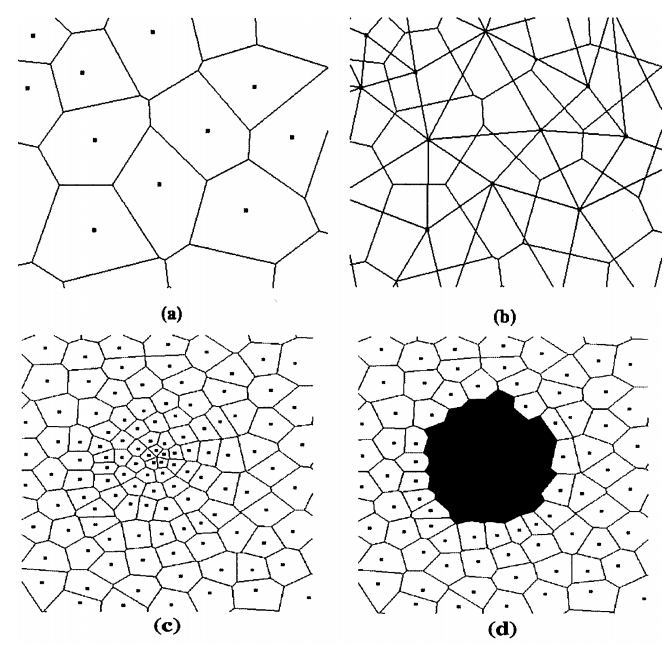
\includegraphics[scale=0.7]{figures/modelado_tamanio}
\caption{Triangulación de Delaunay junto a Polígonos de Thiessen o diagramas de Voronoi para modelizar el tamaño de las células.}
\label{fig:delaunay}
\end{figure}

\newpage

Realizan también un modelado temporal, para así estudiar la velocidad de crecimiento de los tumores.
Sus resultados están muy especializados en un tipo de tumor, por lo que no realizan un estudio genérico
para varios tipos de tumores, con diferentes parámetros, configuraciones o marcadores.


		\chapter{Modelo de eventos}
		Los autores, José Santos y Ángel Monteagudo, decidieron utilizar un autómata celular
siguiendo un modelo de eventos. Es decir, por un lado, la simulación se realiza
sobre una rejilla en tres dimensiones, comenzando con una única célula en el centro de la misma.
Por otro lado, se programan una serie de eventos para cada una de las células de la rejilla, aleatoriamente
entre 5 y 10 (ambos inclusive) iteraciones en el futuro.

Las características y propiedades del sistema se describen en las secciones de este capítulo que
se muestran a continuación.

\section{Las células, genoma y propiedades}

Cada célula estará alojada en una única posición del autómata. En esta simulación, no se modeliza
el tamaño de las células, es decir, aunque en las células cancerosas se observa, además de un comportamiento
replicativo sin control, un crecimiento en su tamaño sin control, los autores no han tenido en cuenta esto.

El genoma de cada célula presente en la rejilla cuenta con un genoma y unas propiedades únicas para cada una de ellas.
En cuanto a su genoma, cuenta con 5 variables binarias que representan la presencia o no de una mutación, la cual, define
un determinado comportamiento canceroso. Estas mutaciones son las siguientes:

\begin{itemize}
    \item \textbf{SG}: Autogeneración de los mensajes de crecimeinto. Esto es, la mutación que permite que la
    célula genere sus propios mensajes para ejecutar la división con idependencia externa.
    \item \textbf{IGI}: Inibhición de las señales de anticrecimiento. Esto es, ante la recepción de una orden
    de detener su crecimiento, la célula tiene una mutación que le permite un mecanismo de ignorancia de los mismos.
    \item \textbf{EA}: Evasión de apoptosis. Esto es, la célula puede, mediante mutación, no hacer caso ante
    una orden de apoptosis, o muerte celular controlada.
    \item \textbf{EI}: Inmortalidad efectiva. Esto es, la célula adquiere una mutación que permite evitar un límite
    replicativo existente, entre otros factores, por el tamaño del telómero.
    \item \textbf{GI}: Inestabilidad genética. Esto es, una mutación que permite a la célula acumular más daño genético, es decir,
    la tasa de mutación base se va incrementando con el paso del tiempo.
\end{itemize}

Además, cada célula tiene una tasa de mutación base y un tamaño de telómero. El primero, es utilizado a la hora
de añadir nuevas mutaciones a la célula. Y la segunda, es un límite replicativo debido a que el ADN queda
desprotegido para futuras mutaciones y podrían ocurrir errores.

\section{Parámetros globales}

De cara a la simulación, existen una serie de parámetros globales que inciden en determinados mecanismos de la misma y
, por tanto, afectan en la evolución de la misma. Esto son:

\begin{itemize}
    \item \textbf{t}: Tamaño de la rejilla.
    \item \textbf{m}: Valor por defecto que indica la tasa de mutación base de cada célula al inicio.
    \item \textbf{tl}: Valor por defecto que indica el tamaño del telómero de cada célula al inicio.
    \item \textbf{e}: Valor por defecto utilizado para definir la probabilidad de una célula de morir por daño genético.
    \item \textbf{i}: Valor por defecto utilizado como factor de aumento de la tasa de mutación base de las células.
    \item \textbf{g}: Valor por defecto para ver qué probabilidad hay de que una célula cancerosa mate a un vecino para
    poder reproducirse.
    \item \textbf{a}: Valor por defecto para ver con qué probabilidad una célula muere de forma aleatoria. Este parámetro
    se introduce como forma de simular las muy diversas causas que pueden originar en la muerte de la célula, por ejemplo,
    recibir una alta dosis de radiación entre otras.
\end{itemize}

\section{Pruebas previas a la mitosis}

El modelo de eventos, a la hora de realizar la mitosis (división celular), realiza tres pruebas:

\begin{itemize}
    \item \textbf{Prueba de muerte aleatoria}: La célula muere con una probabilidad dada ($1/a$).
    \item \textbf{Prueba de daño genético}: A mayor cantidad de mutaciones, mayor probabilidad de
    que la célula muera ($n/e$, donde n es el número de mutaciones de la célula). Excepto, que
    la célula tenga la mutación $EA$ presente en su genoma.
    \item \textbf{Prueba de mitosis}: En realidad, se trata de tres pruebas cuyo resultado debe
    ser positivo para que la célula pueda ejecutar la mitosis:
    \begin{itemize}
        \item \textbf{Comprobación del factor de crecimiento}: La célula sólo puede realizar la
        mitosis si se encuentra dentro de un límite espacial predefinido. Es decir, hay suficiente
        factor de crecimiento. Fuera de este área no podrá realizar la mitosis, excepto si el
        marcador $SG$ está activo.
        \item \textbf{Comprobación de ignorancia de inhibición de crecimiento}: Si no hay
        espacio en el vecindario, la célula no podrá realizar la división. Excepto, que
        la mutación $IGI$ esté presente, en cuyo caso, reemplazará a un vecino con una
        probabilidad dada ($1/g$).
        \item \textbf{Comprobación de potencial replicativo sin límites}: .
    \end{itemize}
\end{itemize}

En estas pruebas, se utilizan los parámetros globales, además, de las propiedades y el genóma de la célula.

\section{Equivalencia temporal}

El ciclo de vida de las células biológicas es de entre 15 y 24 horas. Este ciclo se divide en 5 fases, que son:
fase G0, fase G1, fase S, fase G2 y fase M.

Una célula parte en fase de reposo (G0). Si hay espacio suficiente a su alrededor (vecindario) automáticamente pasa
a fase G1. En la simulación, G1 se simula mediante el paso del tiempo (iteraciones) y la programación de
eventos mitóticos en el futuro (entre 5 y 10 iteraciones, ambas inclusive). Además, en la simulación no se
tiene en cuenta el crecimiento celular.

La fase S es cuando tiene lugar la replicación del ADN. La cual, puede introduccir una mutación ocasionalmente.
La célula entra en una última fase previa a la mitosos, llamada fase G2, en la cual se producen una serie
de comprobaciones sobre el daño genético. Esto, puede provocar la apoptosis (muerte celular programada) en la célula.

Finalmente, la célula entra en la fase M o de mitosis. Todo este ciclo, que en la simulación toma entre 5 y 10 iteraciones
(15 y 24 horas en células biológicas) da una media de 2,6 horas por iteración. Por ejemplo, para 5000 iteraciones se tienen
unas 77,4 semanas aproximadamente.

\section{Bucle principal del modelo de eventos}


		\chapter{Implementación del sistema}
		En este capítulo, se detalla el diseño e implementación del sistema. Tecnologías utilizadas, arquitectura
y diseño, así como, detalles de implementación y patrones que se han seguido.

\section{Tecnologías}

Este proyecto ha sido desarrollado empleando diversas tecnologías y soluciones de $Python$.

$Python$\footnote{\url{https://www.python.org/}} es un lenguaje multiparadigma que es ampliamente utilizado en ámbitos científicos y de investigación.
Cuenta con multitud de herramientas para la realización de $tests$, gestión de dependencias, etc., entre las
que se encuentran $Unittest$\footnote{\url{https://docs.python.org/3/library/unittest.html}} (tests unitarios) y $Pip$\footnote{\url{https://pypi.python.org/pypi/pip}} (gestor de dependencias), que han sido empleadas en este trabajo.

Se ha optado por utilizar el lenguaje de programación $Python$, en su versión 3, concretamente, en el momento de la realización de este trabajo el desarrollo se ha realizado
bajo la versión 3.6.2 de dicho lenguaje.

La implementación de $Python$ utilizada es $CPython$\footnote{\url{https://www.toptal.com/python/por-que-hay-tantos-pythons/es}}.

Además, se han empleado los siguientes paquetes:

\begin{itemize}
  \item \textit{NumPy} como librería fundamental para computación científica del ecosistema \textit{SciPy}.
  \item \textit{Matplotlib} como librería para creación de gráficas del ecosistema \textit{SciPy}.
  \item \textit{Plotly} como librería gráfica, utilizada en este caso sólo para representar figuras en tres dimensiones.
\end{itemize}

Por último, para su desarrollo, se han utilizado otras herramientas como: \textit{Git} y \textit{Git-flow}, \textit{Github},
\textit{Travis}, \textit{Landscape}, \textit{Coveralls} y \textit{Docker}.

\section{Arquitectura y diseño}

Para el desarrollo de este proyecto se ha optado por seguir dos paradigmas simultáneamente. Por un lado,
se ha seguido el paradigma orientado a objeto, esto es, modelizar las partes del sistema con objetos que encapsulan
las propiedades y métodos necesarios según las necesidades u objetivos de cada una de ellas y, las cuales,
se describen en la siguiente sección de este capítulo. Por otro lado, se ha seguido el paradigma funcional, esto es,
diseñar el sistema, o partes de él, en forma de funciones, las cuales para ejecutar su lógica utilizan únicamente
los parámetros que recibe.

\begin{figure}[h]
\centering
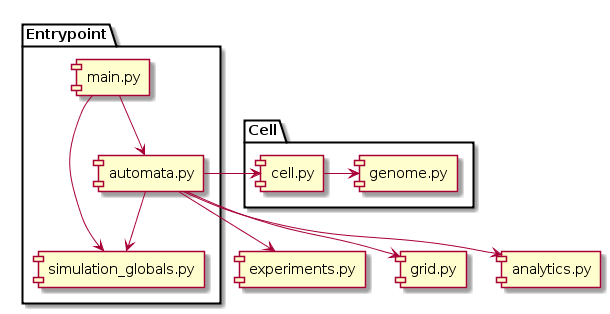
\includegraphics[scale=0.8]{figures/architecture}
\caption{Diagrama de componentes del sistema.}
\label{fig:arch}
\end{figure}

Ambos paradigmas, comentado brevemente en el párrafo anterior, tienen muchos más aspectos, enfoques y soluciones
de las que se comentan. El programa cuenta con un único punto de entrada, como se muestra en la figura~\ref{fig:arch},
en este caso, siguiendo el patrón
\textit{Singleton}. En cuanto a los patrones utilizados, se van a describir en la siguiente sección de este
capítulo donde se presentan los diferentes módulos del mismo.

\section{Módulos del sistema}

En este caso, se han implementado $6$ módulos, como se puede ver en la figura~\ref{fig:arch}.
El módulo principal, \textit{automata.py}, presenta
una clase que sigue el patrón \textit{Estrategia} y, el cual, engloba la función principal de ejecución,
así como, el resto de funciones necesarias para su correcta ejecución. Además, importa y utiliza
el resto de módulos, los caules, se describen a continuación.

\subsection{Módulo \textit{genome.py}}

Este es el primero de los módulos que se ha desarrollado, y es el más simple de todos. Consta de
una clase que contiene únicamente cinco variables binarias, una por cada mutación que se
modeliza en este sistema.

Como se ha descrito previamente, las mutaciones que contiene esta clase son las siguientes:

\begin{itemize}
    \item \textbf{SG}: Autogeneración de los mensajes de crecimiento. Esto es, la mutación que permite que la
    célula genere sus propios mensajes para ejecutar la división con independencia externa.
    \item \textbf{IGI}: Inhibición de las señales de anticrecimiento. Esto es, ante la recepción de una orden
    de detener su crecimiento, la célula tiene una mutación que le permite un mecanismo de ignorancia de los mismos.
    \item \textbf{EA}: Evasión de apoptosis. Esto es, la célula puede, mediante mutación, no hacer caso ante
    una orden de apoptosis, o muerte celular controlada.
    \item \textbf{EI}: Inmortalidad efectiva. Esto es, la célula adquiere una mutación que permite evitar un límite
    replicativo existente, entre otros factores, por el tamaño del telómero.
    \item \textbf{GI}: Inestabilidad genética. Esto es, una mutación que permite a la célula acumular más daño genético, es decir,
    la tasa de mutación base se va incrementando con el paso del tiempo.
\end{itemize}

Además, expone un método que permite obtener el número de mutaciones que tiene cada instancia
de este tipo.

En definitiva, se trata de una clase que, por composición, estará contenida dentro de otra clase
que modeliza a la célula, representando su genoma, y que se explica a continuación.

\subsection{Módulo \textit{cell.py}}

El siguiente módulo, partiendo de la clase genoma, es el que contiene la clase que modeliza
a cada una de las células de la simulación.

Como se ha comentado previamente contiene, por composición, un atributo que representa
al genoma de la célula y que se trata de un objeto tal y como se ha descrito en la sección anterior de este capítulo.
Además, presenta algunos atributos más necesarios para la simulación, y son:

\begin{itemize}
    \item Atributo que representa el tamaño del telómero.
    \item Atributo que representa la tasa de mutación de la célula.
    \item Atributo que representa su posición en la rejilla, es decir, un conjunto de tres elementos
    que representan su posición en cada una de las dimensiones ($(x,y,z)$).
\end{itemize}

Por último, cuenta con varios métodos necesarios para la simulación, y son los siguientes:

\begin{itemize}
    \item \textit{decrease\_telomer()}: Método que se encarga de cambiar el estado interno del objeto, realizando un decrecimiento en una unidad del telómero.
    \item \textit{increment\_base\_muration\_rate(i)}: Las células ven alterada su tasa de mutación base, utilizada para originar nuevas mutaciones durante la mitosis,
    con la presencia de la mutación asociada a la inestabilidad genética o $GI$. Este método realiza este proceso de acuerdo a una tasa de modificación, o incremento,
    de esta tasa, la cual es recibida por parámetros.
    \item \textit{mutations()}: Método que devuelve el número de mutaciones que tiene la célula en su genoma.
    \item \textit{add\_mutations()}: Método que se encarga de generar las nuevas mutaciones que pueden tener lugar durante la mitosis.
    \item \textit{perform\_mitosis()}: El proceso de mitosis queda modelado en este método, esto es, incrementar tasa de mutación base, añadir nuevas mutaciones y
    realizar una copia de sí misma.
\end{itemize}

\subsection{Módulo \textit{simulation\_globals.py}}

De cara a realizar la simulación son necesarios una serie de parámetros que se necesitarán manipular
para realizar los experimentos que se describirán en capítulos posteriores. Esto lleva al siguiente módulo,
en el cual se tiene una clase que contiene sólo atributos que almacenan todos estos parámetros.

Dichos parámetros son los siguientes:

\begin{itemize}
    \item Tasa de mutación base o \textit{m}.
    \item Tamaño del telómero o \textit{tl}.
    \item Probabilidad de evasión de apoptosis o \textit{e}.
    \item Factor de incremento de la tasa de mutación base o \textit{i}.
    \item Probabilidad de matar a un vecino para realizar la mitosis o \textit{g}.
    \item Probabilidad de muerte aleatoria de la célula o \textit{a}.
    \item Límite espacial predefinido.
    \item Límite inferior para evento mitótico en el futuro.
    \item Límite superior para evento mitótico en el futuro.
\end{itemize}

En este fichero, además, se encuentran los valores por defecto de la simulación según los autores
del artículo \cite{jsantos-amonteagudo-1-2014} en el que se basa este trabajo. En este caso,
se declaran como constantes, ya que estos, en caso de ser utilizados en la simulación, no varían.

\subsection{Módulo \textit{experiments.py}}

Para realizar la mitosis, se necesitan realizar varias pruebas o experimentos. Estos
están contenidos dentro de una clase como métodos. Los parámetros necesarios para ejecutar dichas
pruebas se reciben por parámetros. Los métodos, son los siguientes:

\begin{itemize}
  \item \textit{random\_death\_test()}: Prueba que indica si hay o no muerte aleatoria de la célula.
  \item \textit{random\_death\_test(n, ea)}: Prueba que indica si hay muerte por daño genético según
  el número de mutaciones de la célula que está realizando el proceso de mitosis, excepto que esté
  presente el marcador con la mutación que permite evadir la apoptosis.
  \item \textit{random\_death\_test(sg, spatial\_boundary)}: Prueba que está dentro del
  límite espacial o, lo que es lo mismo, si existe suficiente factor de crecimiento como
  para ejecutar la mitosis. Excepto, si tiene presente el marcador $sg$, que permite
  ejecutar la mitosis si la célula se encuentra fuera de dicho espacio.
  \item \textit{random\_death\_test(igi)}: Prueba que comprueba si existe espacio para ubicar la célula
  hija una vez realizada la mitosis. Si no hay espacio y la célula tiene la mutación asociada al
  marcador $igi$, podrá matar a un vecino para ubicar a la célula hija.
  \item \textit{random\_death\_test(tl, ei)}: Prueba que comprueba si el telómero tiene tamaño
  mayor a $0$ para realizar la mitosis. Si el tamaño es $0$, la célula puede realizar mitosis
  si tiene presente la mutación asociada al marcador $ei$.
\end{itemize}

\subsection{Módulo \textit{grid.py}}

El módulo \textit{grid.py} almacena la información relativa a la rejilla en la que tiene lugar
la simulación. Esto es, tiene como propiedad o atributos el ancho, alto y largo del mismo.

Pero, la parte útil de este módulo son los métodos que permiten a la simulación obtener el vecindario,
controlando sus límites, y obtener qué celdas del vecindario están ocupadas y cuales no. Por tanto,
sus métodos son los siguientes:

\begin{itemize}
  \item \textit{neighborhood(origin, radio)}: Método que recibe un centro de tipo $(x,y,z)$ y un radio, para devolver una lista con las posiciones
  que conforman el vecindario.
  \item \textit{filter(value, limit)}: Método que permite saber si un valor está dentro de un límite espacial. Es utilizada en únicamente en el siguiente métodos.
  \item \textit{check\_limits(cube, limit)}: Método que comprueba que, de una lista de posiciones que conforman el vecindario, no existe una posición que exceda el
  límite de la rejilla. Devuelve, la lista sin dichas posiciones.
  \item \textit{classify\_neighborhood(cube, cells)}: Métdodo que clasifica las células de un cubo que representa un vecindario en función de las posiciones
  ocupadas y las que están libres.
\end{itemize}

\subsection{Módulo \textit{automata.py}}

Módulo principal del sistema que contiene la lógica de ejecución del mismo~\ref{fig:automata}. El sistema
está diseñado siguiendo el patrón \textit{Singleton}, es decir, sólo hay un objeto
autómata que, implementando el patrón \textit{estrategia}, tiene un, método con
la lógica de ejecución.

La lógica de ejecución se encuentra descrita en la sección 4.8 de este documento.

Además, tiene como atributos la agenda de eventos mitóticos, así como, el objeto que
encapsula los experimentos necesarios para saber si se aplica o no mitosis a cada célula, los
parámetros de simulación, el objeto con la lógica necesaria para gestionar la rejilla y, por último,
la responsabilidad de generar las medidas utilizando el módulo de analítica que se describe a continuación.

\begin{figure}[h]
\centering
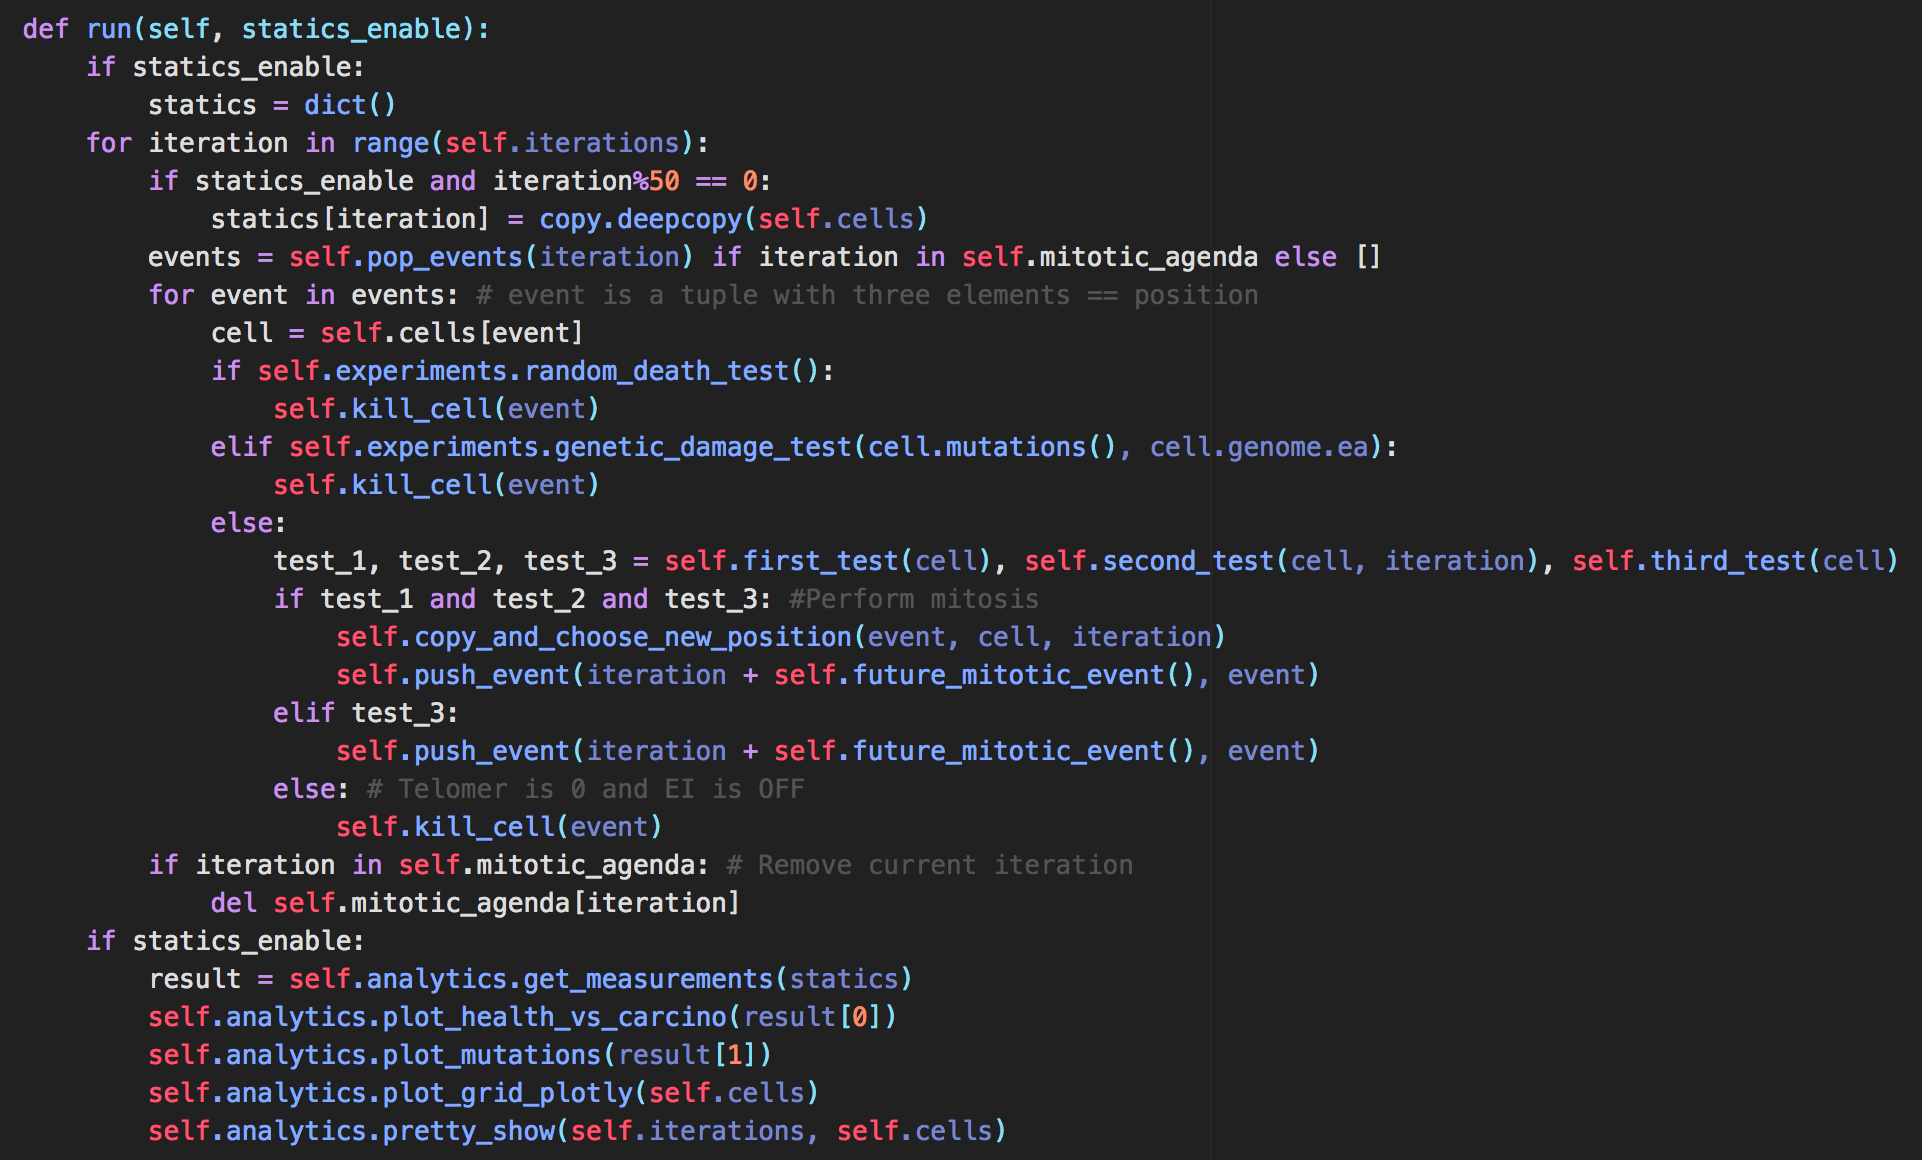
\includegraphics[scale=0.45]{figures/alg}
\caption{Código con el bucle principal de la simulación.}
\label{fig:automata}
\end{figure}

\subsection{Módulo \textit{analytics.py}}

Este último módulo, reúne las funciones necesarias para hacer medidas sobre las células
de la rejilla, como por ejemplo, células sanas o cancerígenas, cuántas células tienen un
determinado marcador del cáncer activo, etc.

Además, contiene funciones para construir y mostrar gráficas con vista a presentar la evolución
del sistema a lo largo de la simulación.

\section{Instalación y ejecución}

En esta última sección del capítulo dedicado a la implementación, se expone la información necesaria
para su instalación y uso. Existen dos formas de conseguirlo, la primera, a través de una ejecución
nativa, es decir, sobre la propia máquina local. En segundo lugar, sobre \textit{Docker}, lo cual permite
no realizar ninguna instalación sobre la máquina local.

\subsection{Prerrequisitos}

Dependiendo del tipo de instalación, se dan los siguientes prerrequisitos:

\begin{itemize}
  \item Para una ejecución sobre la máquina local, se necesita:
        \item Instalar la versión 3.6+ de \textit{Python}\footnote{\url{https://www.python.org/downloads/}}.
        \item Instalar el gestor de paquetes de \textit{Python}, \textit{pip}\footnote{\url{https://pip.pypa.io/en/stable/installing/}}.
        \item Instalar el control de versiones \textit{Git}\footnote{\url{https://git-scm.com/book/en/v2/Getting-Started-Installing-Git}}.
        \item Clonar el repositorio ejecutando en consola \textit{git clone \url{https://github.com/MULCIA/TFMSTGCA.git}}.
        \item Instalar dependencias con \textit{pip}, para ello, ejecutar en consola \textit{pip install -r requirements.txt}.
  \item Para una ejecución con \textit{Docker} se necesita:
        \item Instalar la última versión de \textit{Docker}\footnote{\url{https://docs.docker.com/engine/installation/}}.
        \item Instalar el control de versiones \textit{Git}\footnote{\url{https://git-scm.com/book/en/v2/Getting-Started-Installing-Git}}.
        \item Clonar el repositorio ejecutando en consola \textit{git clone \url{https://github.com/MULCIA/TFMSTGCA.git}}.
\end{itemize}

\subsection{Ejecución}

Dependiendo del modo elegido, es decir, ejecución en máquina local o ejecución en \textit{Docker}, su ejecución es diferente.

En primer lugar, se describe como hacer una ejecución en máquina local. Una vez cumplidos los requisitos descritos anteriormentes,
para ejecutar el proyecto sólo hay que ejecutar, dentro del directorio que contiene el proyecto, el siguiente comando:
\textit{python main.py}.

Su ejecución se realiza automáticamente y al finalizar mostrará una serie de gráficas:

\begin{itemize}
  \item Gráfica que muestra la evolución en número de las células sanas frente a las células cancerosas.
  \item Gráfica que muestra la evolución en número de los marcadores.
  \item Gráfica que muestra la rejilla en tres dimensiones mostrando las células sanas (gris) y las células cancerosas (verde).
\end{itemize}

En segundo lugar, se describe como hacer la ejecución en \textit{Docker}. Una vez cumplido los requisitos anteriores, existen dos
formas de ejecutar la simulación: ejecutar los comandos de docker, o emplear unos scripts que se encuentran embebidos en el proyecto.
Dichos scripts sólo se pueden emplear de tratarse de una máquina \textit{Linux}.

\clearpage

Los comandos de consola de \textit{Docker} son los siguientes:

\begin{itemize}
  \item Para construir la imagen: \textit{docker build -t TFMSTGCA/tfm . }.
  \item Para levantar el contenedor: \textit{docker run --name tfm -d TFMSTGCA/tfm:latest tail -f /dev/null}. Se ejecuta en modo demonio y se mantiene su
  ejecución. Al finalizar el proceso de creación y ejecución del contenedor, se realiza una ejecución de los tests adjuntos al proyecto.
  \item Para ejecutar la simulación: \textit{docker exec -it tfm bash}. Una vez ejecutado, con la terminal del contenedor en la consola, ejecutar como se describe previamente
  para la ejecución en máquina local.
\end{itemize}

\subsection{Parámetros de la simulación}

La simulación cuenta con la posibilidad de ajustar los parámetros que se describen en la sección anterior,
donde se comenta el módulo \textit{simulation\_globals.py}. En el punto de entrada de la aplicación,
en \textit{main.py}, se encuentra la declaración del objeto \textit{SimulationGlobals}.

Para realizar ajustes, existen dos formas:

\begin{itemize}
  \item Utilizar la configuración por defecto de los autores.
  \item Utilizar una configuración propia.
\end{itemize}

Para el primer caso, se cuenta con una serie de constantes que permiten dejar el sistema con la
configuración por defecto que dan los autores.

Para el segundo caso, sólo hay que establecer el parámetro deseado sustituyendo cualquiera de las constantes. Esto es,
modificar en el fichero \textit{main.py} la primera línea del programa, que aparece de la siguiente forma:
\textit{simulationGlobals = SimulationGlobals(...)}.
Para la configuración del autómata modificar la siguiente línea en el fichero \textit{main.py}, esto es,
la línea \textit{automata = Automata(50, 50000, simulationGlobals)}, donde el primer parámetro es el tamaño
para la rejilla, el segundo el número de iteraciones de la simulación y, por último, los parámetros que se han
descrito previamente.


		\chapter{Experimentos de los autores}
		José Santos y Ángel Monteagudo realizaron una serie de simulaciones en su artículo
donde intentan estudiar la influencia de los marcadores en la evolución de la simulación.
Todas las simulaciones, y sus resultados, se comentan en esta sección.

El tamaño de rejilla utilizada para todos los experimentos es de $50^3$. Esto son,
$125.000$ células posibles en la rejilla.

\section{Influencia del parámetro \textit{Tasa de mutación base (m)}}

Los autores en su artículo presentan 3 experimentos utilizando los valores por defecto
y variando el parámetro \textit{Tasa de mutación base (m)} para estudiar como afecta
dicho parámetro en la proliferación del cáncer.

Cada experimento se muestra en una serie de gráficas en las cuales se presenta
como resultado la media de 5 ejecuciones diferentes.

A continuación, se muestra cada uno de los experimentos especificando en cada caso
el valor $m$ utilizado. El resto de parámetros de la simulación se mantiene constante
con los valores considerados por defectos, que son:

\begin{table}[h!]
  \centering
  \caption{Valores de los parámetros, excepto \textit{m}.}
  \label{tab:table1}
  \begin{tabular}{ccc}
    \toprule
    Nombre & Símbolo & Valor\\
    \midrule
    Tamaño del telómero & tl & 50\\
    Muerte por daño genético & e & 10\\
    Factor de incremento de tasa de mutación base & i & 100\\
    Muerte de un vecino & g & 30\\
    Muerte aleatoria & a & 1000\\
    \bottomrule
  \end{tabular}
\end{table}

\subsection{Experimento 1: Tasa de mutación base igual a 10.000}

En este primer experimento, los autores presentan un valor para el parámetro
tasa de mutación base de $m=10000$. Realizan una simulación de $1000$ iteraciones.

Es importante recordar, que al utilizar $1/m$ para representar la probabilidad
de que aparezcan diferentes mutaciones al realizar la mitosis, a mayor valor
del parámetro $m$, menor probabilidad de que ocurran mutaciones.

En la simulación, el número de células cancerosas es muy bajo y crece muy levemente,
no superando las $10000$ células de las $125000$ totales. En cuanto a lo marcadores,
el marcador $SG$ toma ventaja y tiene ocurrencia en la mayoría de células cancerosas
(una célula cancerosa es aquella que tiene, al menos, una mutación). El siguiente marcador
presente, aunque con mucha diferencia, es $EA$. El resot de marcadores presenta
un comportamiento similar y su presencia es casi inexistente.

\begin{figure}[h]
\centering
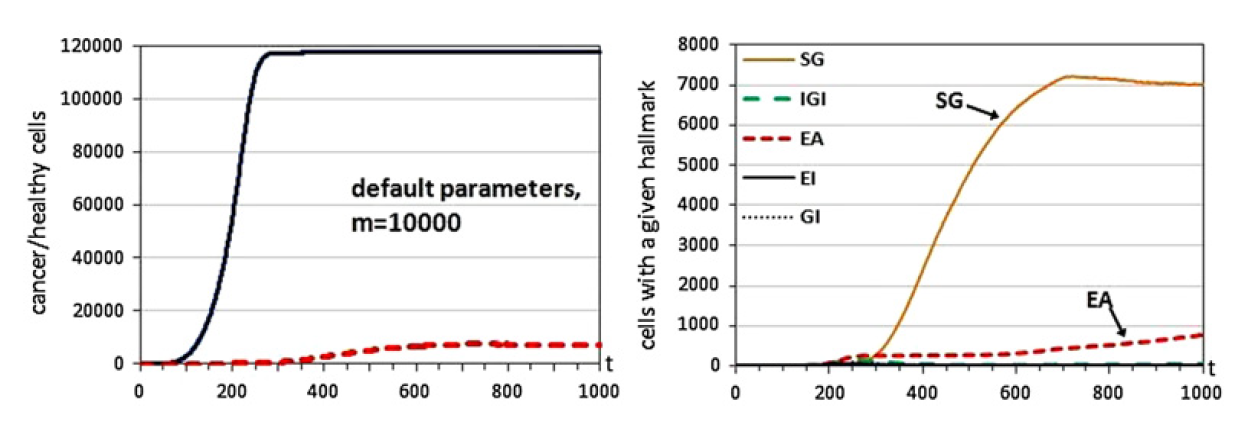
\includegraphics[scale=0.6]{figures/experiments/exp1}
\caption{Completar.}
\end{figure}

\subsection{Experimento 2: Tasa de mutación base igual a 1.000}

En el segundo experimento, los autores alteran el valor para el parámetro tasa de
mutación base a $m=1000$.

Los resultados obtenidos para $1000$ iteraciones presentan varias diferencias. En primer lugar,
el número de células cancerosas aumenta, lo cual, se explica por la mayor probabilidad
de mutaciones provocadas al realizar la mitosis. En segundo lugar, en cuanto a los marcadores,
aparecen todos los marcadores, con un comportamiento bastante similar entre ellos. Se pueden
destacar los marcadores $EA$ y $SG$, que toman algo de ventaja respecto al resto.

\begin{figure}[h]
\centering
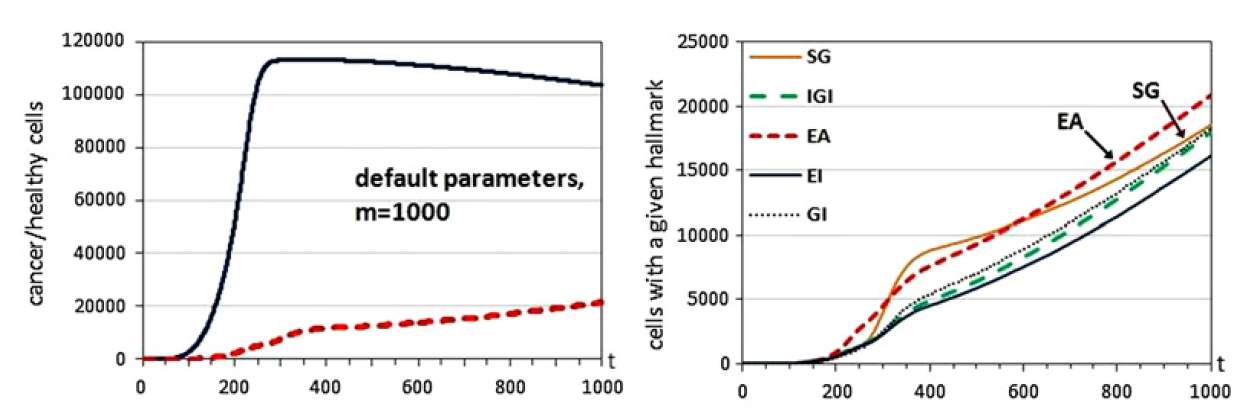
\includegraphics[scale=0.6]{figures/experiments/exp2}
\caption{Completar.}
\end{figure}

\subsection{Experimento 3: Tasa de mutación base igual a 100}

En este tercer y último experimento de este tipo, los autores obtienen cambios relevantes frente a los dos
experimentos anteriores.

En primer lugar, el número de células cancerosas pronto supera a las células sanas, e incluso,
a lo largo de las iteraciones terminan, las células cancerosas, representando casi la totalidad de
la rejilla. Esto se explica por la mayor probabilidad de aparición de mutaciones durante la mitosis, en
este caso, la tasa de mutación base es de $m=100$.

En segundo lugar, en cuanto a marcadores, ocurren todos los marcadores con un comportamiento similar,
tomando ventaja, pero muy levemente, los marcadores $EA$ e $IGI$. La principal diferencia en este punto es
la presencia del marcador $IGI$, el cual, tiene mayor presencia que otros. El marcador $SG$ no toma ventaja en
este punto, como si lo hacía en los dos experimentos anteriores.

El marcador $EA$ siempre está presente y cobra un papel fundamental, ya que, permite la proliferación
de células cancerosas debido a que supone que la célula con dicho marcador puede evadir la muerte
celular programada.

\begin{figure}[h]
\centering
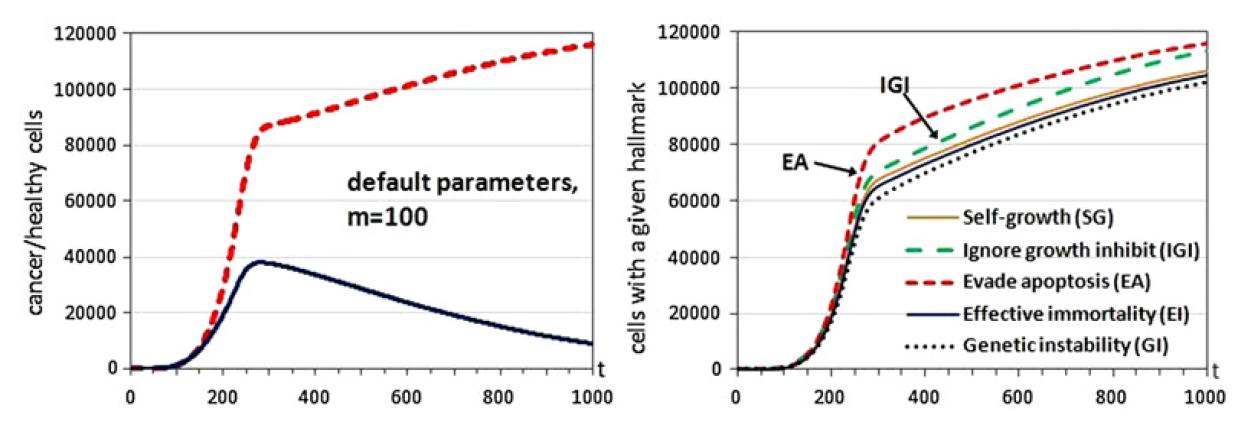
\includegraphics[scale=0.6]{figures/experiments/exp3}
\caption{Completar.}
\end{figure}

\section{Influencia del resto de parámetros}

Los autores realizan un segundo experimento con el objetivo de observar los efectos
que tienen el resto de parámetros sobre la simulación. Para ello, varían los parámetros de
la simulación, como se puede observar en la siguiente tabla:

\begin{table}[h!]
  \centering
  \caption{Valores de los parámetros.}
  \label{tab:table1}
  \begin{tabular}{ccc}
    \toprule
    Nombre & Símbolo & Valor\\
    \midrule
    Tasa de mutación base & m & 100.000\\
    Tamaño del telómero & tl & 35\\
    Muerte por daño genético & e & 20\\
    Factor de incremento de tasa de mutación base & i & 100\\
    Muerte de un vecino & g & 10\\
    Muerte aleatoria & a & 400\\
    \bottomrule
  \end{tabular}
\end{table}

Se observa un comportamiento bastante representativo, por ejemplo, un menor valor
para el número de iteraciones implica menos eventos mitóticos en las células sanas, y
un menor valor del parámetros $a$ facilita la aparición de sitios vacacntes que
quedan disponibles para la propagación de células cancerosas, en conexión con una
mayor probabilidad de reemplazar a un vecino para realizar la mitósis (parámetros $g$).

En la gráfica de evolución de los marcadores se observa que en este caso el marcador
dominante es $EI$. En este caso, se realizan $5000$ iteraciones. El marcador $EI$ implica
la progresión de estas células debido a que evitan la muerte por agotamiento del telómero.
En la simulación, por contra, tener un telómero más corto implica tener menos oportunidades de división, como
ocurre con la célula inicial del centro de la rejilla.

El resto de marcadores aparecen más tarde en la simulación. El siguiente marcador en hacer
presencia es $EA$, lo cual permite a las células evadir la muerte celular programada. Este marcador
también favorece la proliferación del cáncer, por tanto, toma cada vez más ventaja. El marcador
$SG$ aparece algo más tarde que los anteriores y permite proliferar al cancer
fuera del límite reproductivo, por tanto, alcanza un límite y se mantiene estable.

El último marcador en aparecer es $IGI$. No prolifera rápidamente debido a no disponer
de espacio vacante para realizar la división.

\begin{figure}[h]
\centering
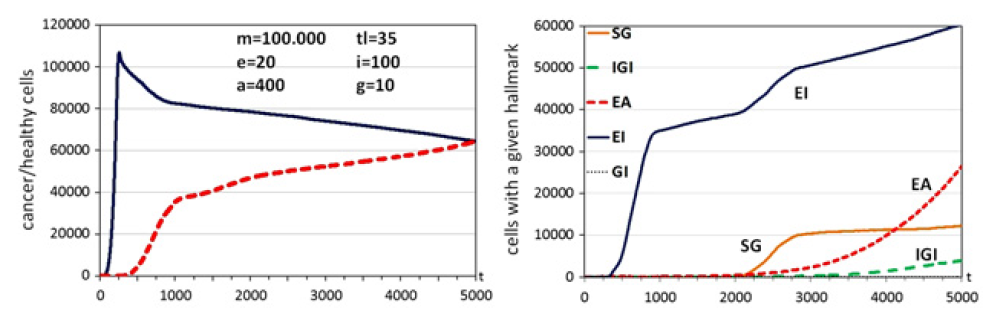
\includegraphics[scale=0.8]{figures/experiments/exp4}
\caption{Completar.}
\end{figure}

\section{Influencia de parámetros con rejilla completa de células sanas}

En este caso, se parte con una rejilla completa de células sanas. En cuanto a los parámetros,
se utilizan los mismos que en la sección anterior.

Se realizan diferentes estrategias en cuanto al número de iteraciones, desde $8000$ iteraciones
hasta $100000$ iteraciones, es decir, la simulación se corresponde con una equivalencia temporal
de $2.3$ años y $29.7$ años respectivamente.

Completar.

\begin{figure}[h]
\centering
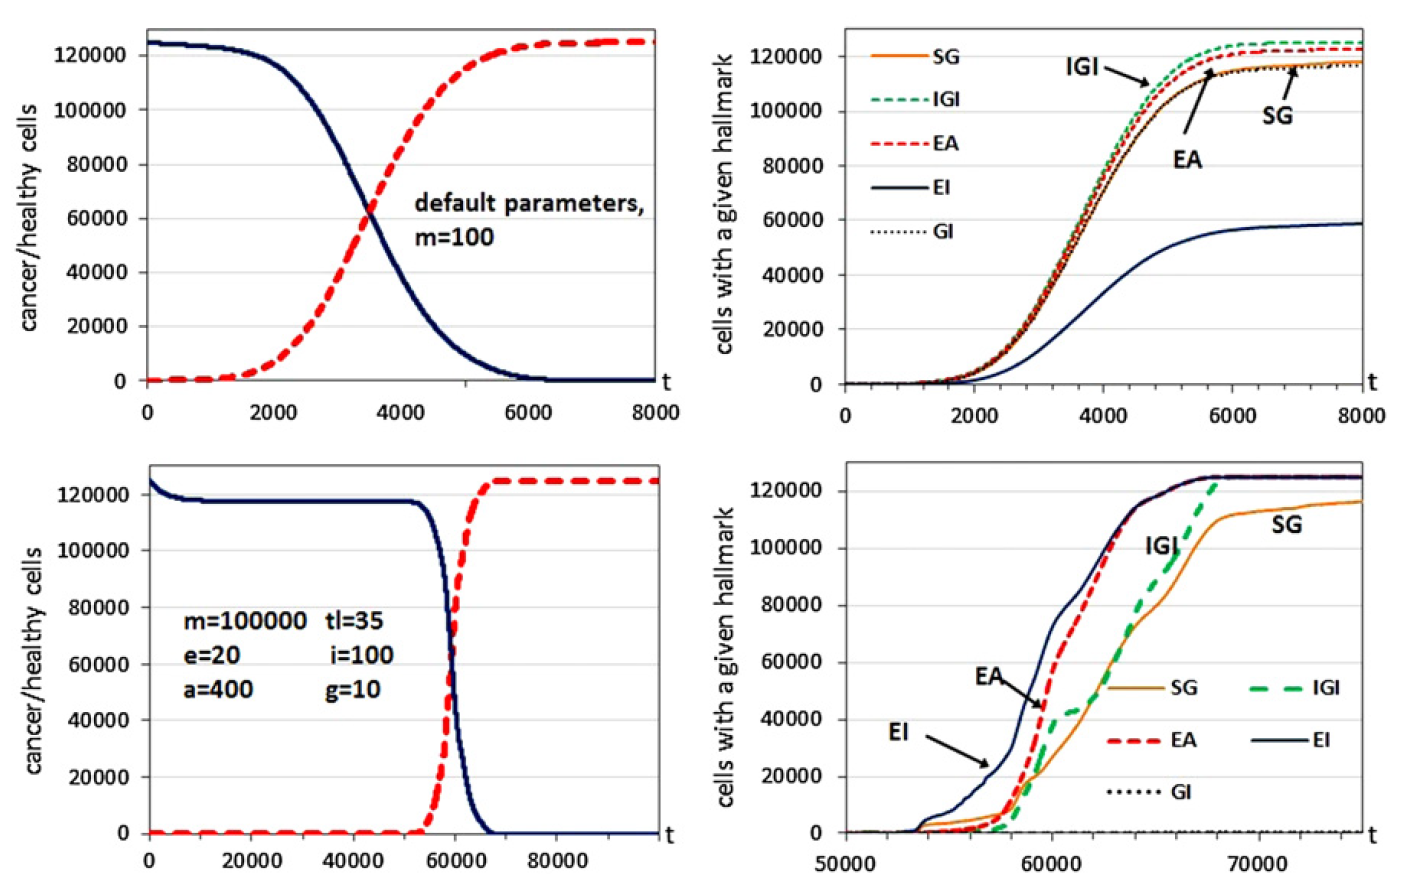
\includegraphics[scale=0.5]{figures/experiments/exp5}
\caption{Completar.}
\end{figure}

\section{Relevancia de los marcadores}

En este caso, los autores intentan responder a la siguiente pregunta: \textit{¿Cuál sería
el comportamiento emergente si algún marcador no estuviera presente y no aplicaran
sus efectos?}.

Conocer el efecto de cada marcador en el comportamiento emergente para crecimiento de tumores
puede resultar útil para mejorar las terapias contra el cáncer.

En su estudio, los autores encuentran el marcador $EA$ o de evasión de apoptosis como el más
relevante de todos, debido a que se reduce drásticamente el número de células cancerígenas.
Tras él, los siguientes marcadores más relevantes por orden son $GI$ o de inestabilidad genética y,
a continuación, $IGI$ o inhibición de señal de parada de crecimiento. Esto se debe a, en el caso
del marcador $GI$, se reducen las posibilidades de adquirir una mutación. Respecto al marcador $IGI$,
esto se debe a que cuando la rejilla no tiene espacio libre, sobre todo con células sanas, se reduce
la probabilidad de, para realizar la división, una célula mate a un vecino para conseguir espacio.

Completar.

\begin{figure}[h]
\centering
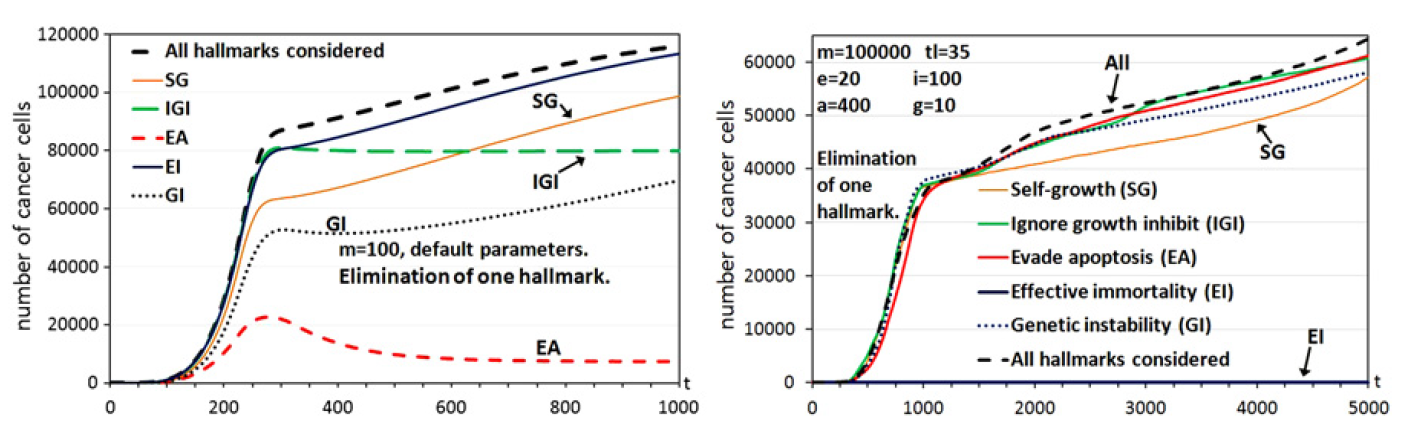
\includegraphics[scale=0.5]{figures/experiments/exp6}
\caption{Completar.}
\end{figure}

\section{Comportamiento de las transiciones}

El objetivo es estudiar el comportamiento de las transiciones cuando un agente actua contra las células cancerosas.
En este caso, la simulación comienza con la rejilla completa de células cancerosas, y se supone una terapia
perfecta, en el sentido que la droga, en este caso, actúa sólo contra las células cancerosas.

Completar.

\begin{figure}[h]
\centering
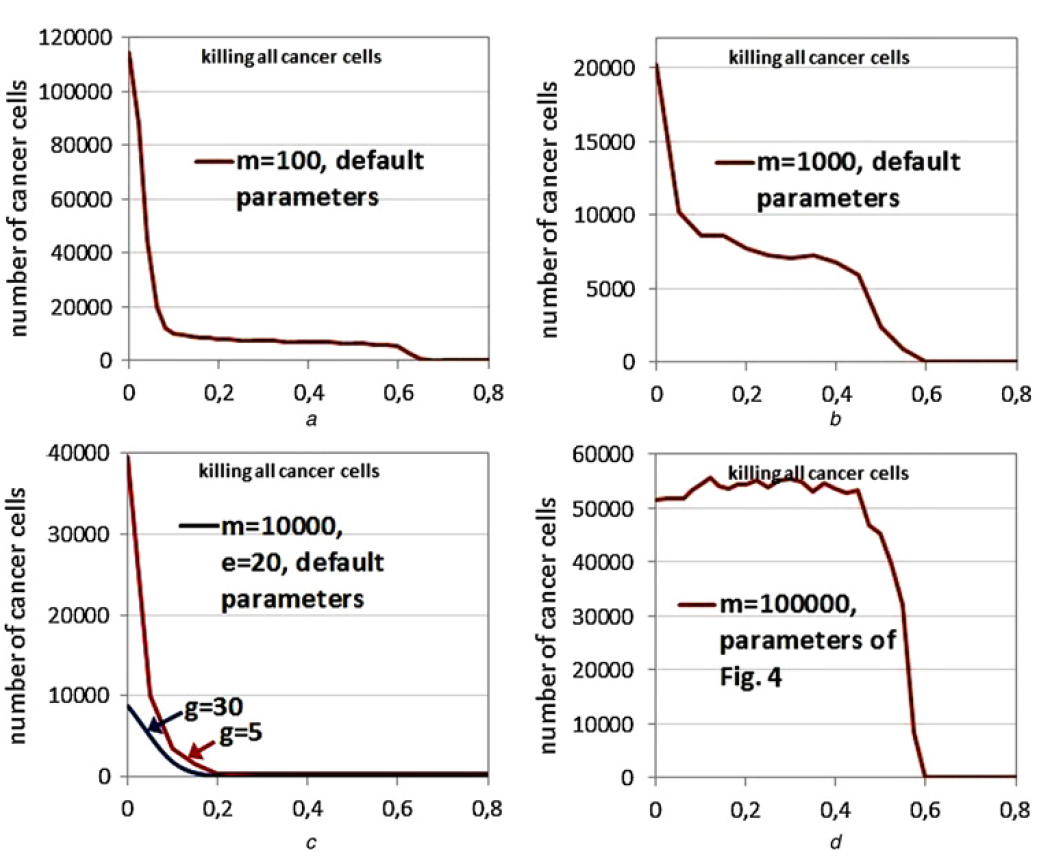
\includegraphics[scale=0.7]{figures/experiments/exp7}
\caption{Completar.}
\end{figure}

\begin{figure}[h]
\centering
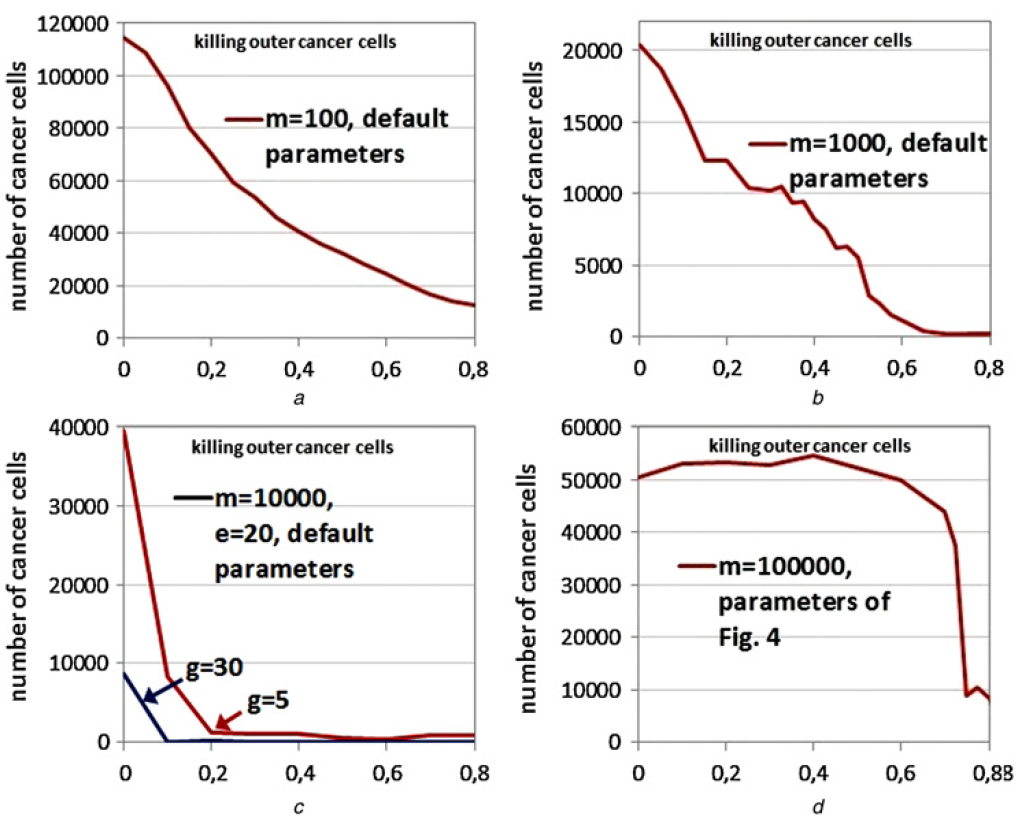
\includegraphics[scale=0.7]{figures/experiments/exp8}
\caption{Completar.}
\end{figure}


		\chapter{Resultados propios}
		Lorem ipsum dolor sit amet, consectetur adipisicing elit, sed do eiusmod tempor incididunt ut labore et dolore magna aliqua.
Ut enim ad minim veniam, quis nostrud exercitation ullamco laboris nisi ut aliquip ex ea commodo consequat.
Duis aute irure dolor in reprehenderit in voluptate velit esse cillum dolore eu fugiat nulla pariatur.
Excepteur sint occaecat cupidatat non proident, sunt in culpa qui officia deserunt mollit anim id est laborum.

\section{Influencia del parámetro \textit{Tasa de mutación base (m)}}

Lorem ipsum dolor sit amet, consectetur adipisicing elit, sed do eiusmod tempor incididunt ut labore et dolore magna aliqua.
Ut enim ad minim veniam, quis nostrud exercitation ullamco laboris nisi ut aliquip ex ea commodo consequat.
Duis aute irure dolor in reprehenderit in voluptate velit esse cillum dolore eu fugiat nulla pariatur.
Excepteur sint occaecat cupidatat non proident, sunt in culpa qui officia deserunt mollit anim id est laborum.

\subsection{Experimento 1: Tasa de mutación base igual a 10.000}

Lorem ipsum dolor sit amet, consectetur adipisicing elit, sed do eiusmod tempor incididunt ut labore et dolore magna aliqua.
Ut enim ad minim veniam, quis nostrud exercitation ullamco laboris nisi ut aliquip ex ea commodo consequat.
Duis aute irure dolor in reprehenderit in voluptate velit esse cillum dolore eu fugiat nulla pariatur.
Excepteur sint occaecat cupidatat non proident, sunt in culpa qui officia deserunt mollit anim id est laborum.

\begin{figure}[h]
\centering
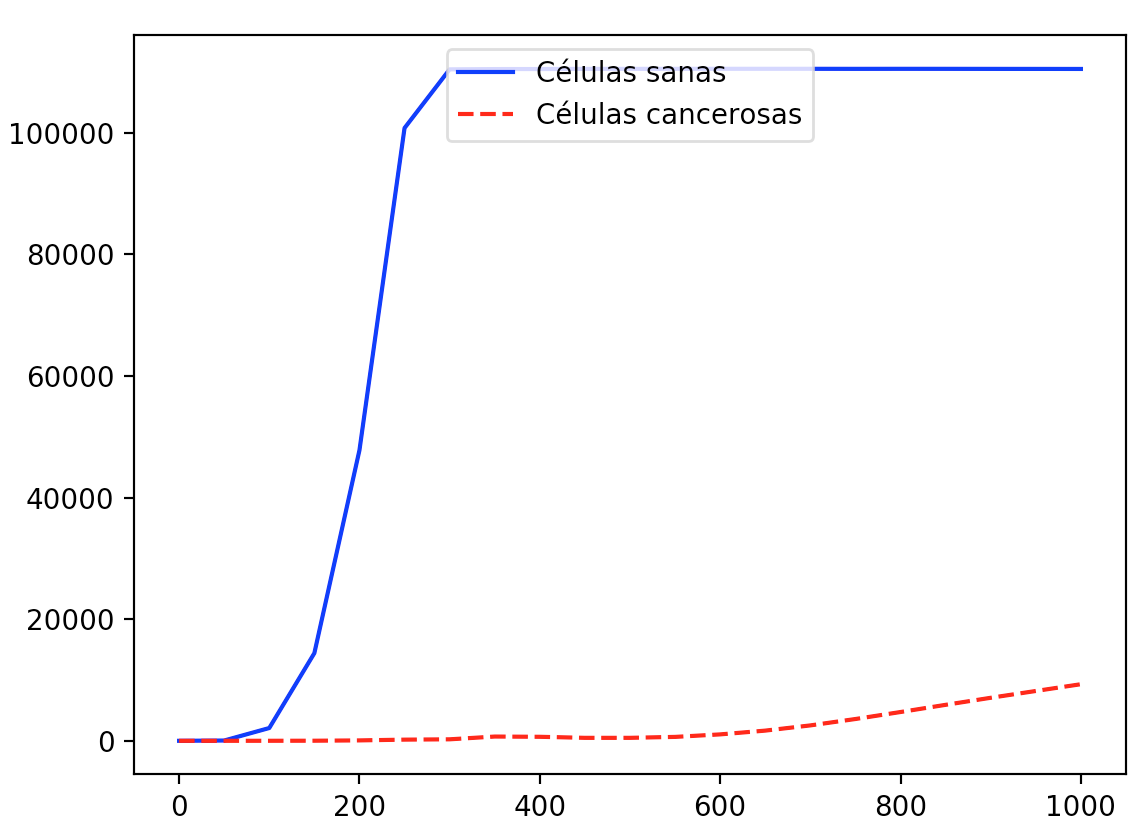
\includegraphics[scale=0.6]{figures/experiments/exp1/healthvscarcino}
\caption{Completar.}
\end{figure}

Lorem ipsum dolor sit amet, consectetur adipisicing elit, sed do eiusmod tempor incididunt ut labore et dolore magna aliqua.
Ut enim ad minim veniam, quis nostrud exercitation ullamco laboris nisi ut aliquip ex ea commodo consequat.
Duis aute irure dolor in reprehenderit in voluptate velit esse cillum dolore eu fugiat nulla pariatur.
Excepteur sint occaecat cupidatat non proident, sunt in culpa qui officia deserunt mollit anim id est laborum.

\begin{figure}[h]
\centering
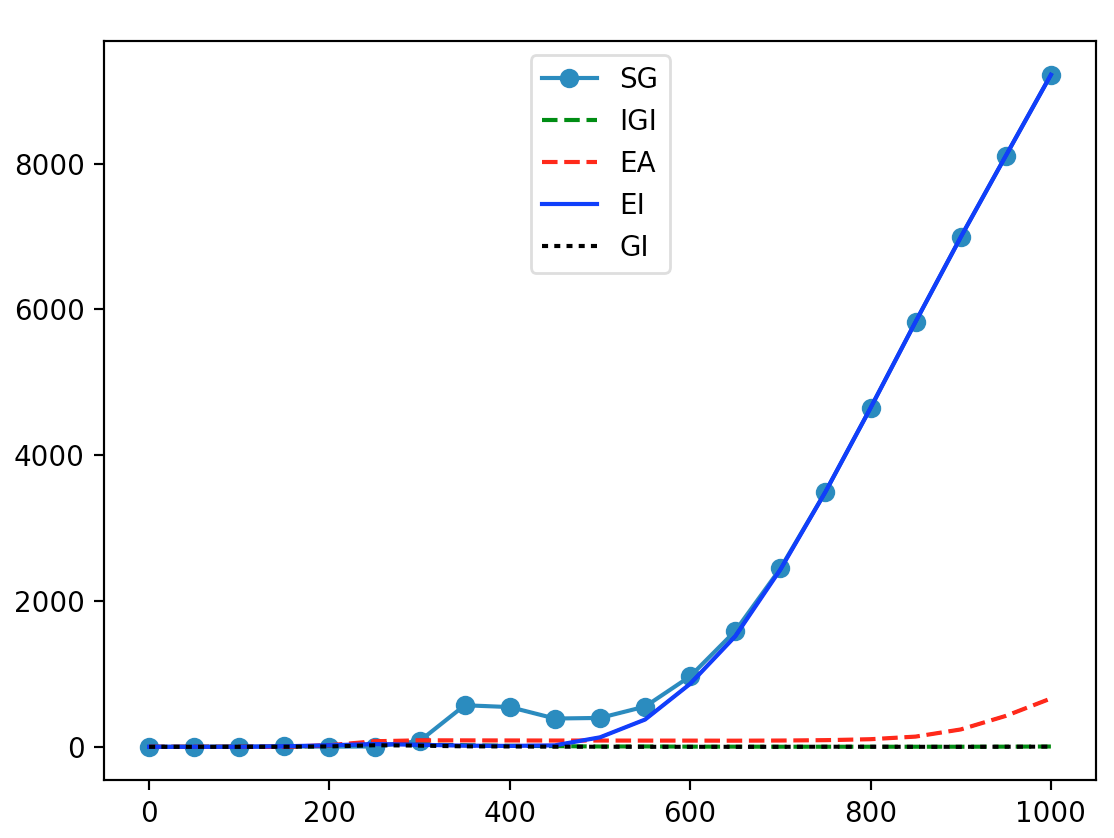
\includegraphics[scale=0.6]{figures/experiments/exp1/mutations}
\caption{Completar.}
\end{figure}

Lorem ipsum dolor sit amet, consectetur adipisicing elit, sed do eiusmod tempor incididunt ut labore et dolore magna aliqua.
Ut enim ad minim veniam, quis nostrud exercitation ullamco laboris nisi ut aliquip ex ea commodo consequat.
Duis aute irure dolor in reprehenderit in voluptate velit esse cillum dolore eu fugiat nulla pariatur.
Excepteur sint occaecat cupidatat non proident, sunt in culpa qui officia deserunt mollit anim id est laborum.

\begin{figure}[h]
\centering
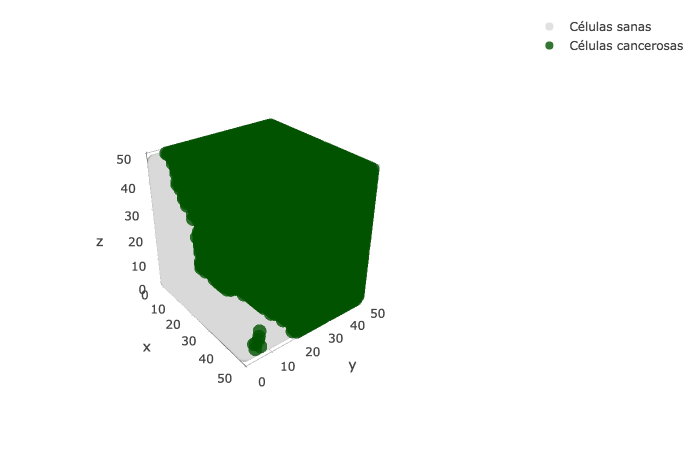
\includegraphics[scale=0.6]{figures/experiments/exp1/grid}
\caption{Completar.}
\end{figure}

Lorem ipsum dolor sit amet, consectetur adipisicing elit, sed do eiusmod tempor incididunt ut labore et dolore magna aliqua.
Ut enim ad minim veniam, quis nostrud exercitation ullamco laboris nisi ut aliquip ex ea commodo consequat.
Duis aute irure dolor in reprehenderit in voluptate velit esse cillum dolore eu fugiat nulla pariatur.
Excepteur sint occaecat cupidatat non proident, sunt in culpa qui officia deserunt mollit anim id est laborum.

\subsection{Experimento 2: Tasa de mutación base igual a 1.000}

Lorem ipsum dolor sit amet, consectetur adipisicing elit, sed do eiusmod tempor incididunt ut labore et dolore magna aliqua.
Ut enim ad minim veniam, quis nostrud exercitation ullamco laboris nisi ut aliquip ex ea commodo consequat.
Duis aute irure dolor in reprehenderit in voluptate velit esse cillum dolore eu fugiat nulla pariatur.
Excepteur sint occaecat cupidatat non proident, sunt in culpa qui officia deserunt mollit anim id est laborum.

\begin{figure}[h]
\centering
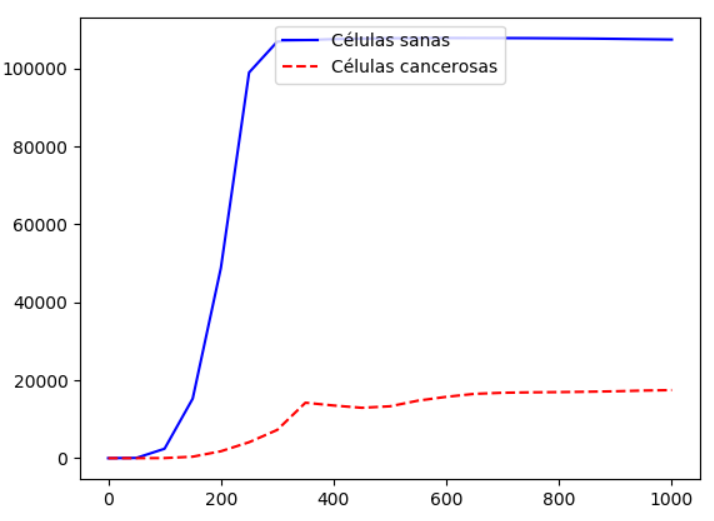
\includegraphics[scale=0.8]{figures/experiments/exp2/healthvscarcino}
\caption{Completar.}
\end{figure}

Lorem ipsum dolor sit amet, consectetur adipisicing elit, sed do eiusmod tempor incididunt ut labore et dolore magna aliqua.
Ut enim ad minim veniam, quis nostrud exercitation ullamco laboris nisi ut aliquip ex ea commodo consequat.
Duis aute irure dolor in reprehenderit in voluptate velit esse cillum dolore eu fugiat nulla pariatur.
Excepteur sint occaecat cupidatat non proident, sunt in culpa qui officia deserunt mollit anim id est laborum.

\begin{figure}[h]
\centering
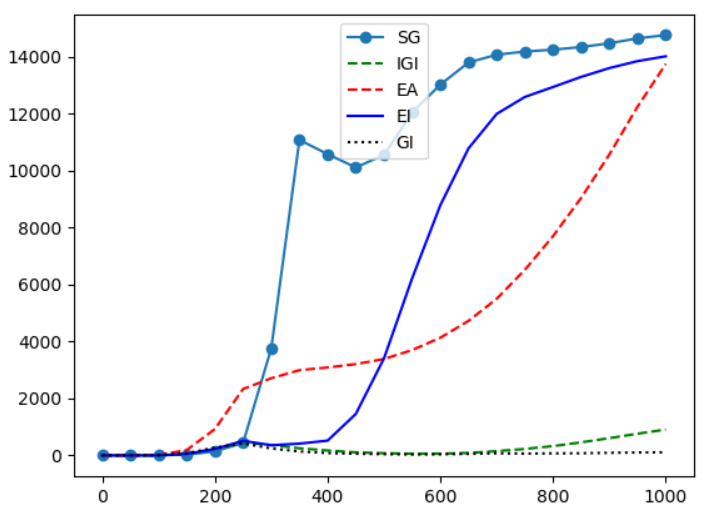
\includegraphics[scale=0.8]{figures/experiments/exp2/mutations}
\caption{Completar.}
\end{figure}

Lorem ipsum dolor sit amet, consectetur adipisicing elit, sed do eiusmod tempor incididunt ut labore et dolore magna aliqua.
Ut enim ad minim veniam, quis nostrud exercitation ullamco laboris nisi ut aliquip ex ea commodo consequat.
Duis aute irure dolor in reprehenderit in voluptate velit esse cillum dolore eu fugiat nulla pariatur.
Excepteur sint occaecat cupidatat non proident, sunt in culpa qui officia deserunt mollit anim id est laborum.

\begin{figure}[h]
\centering
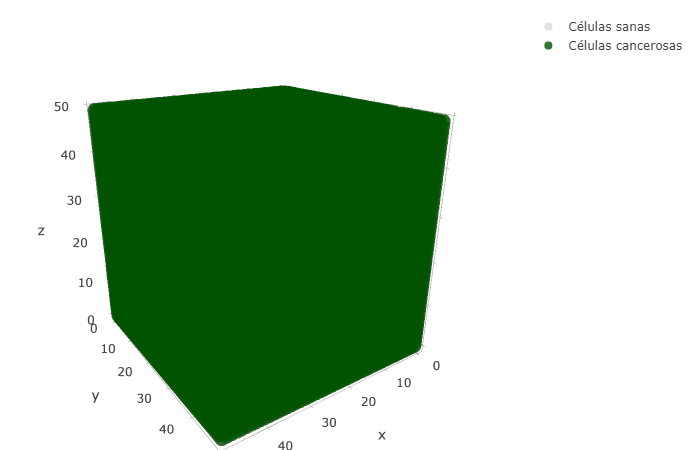
\includegraphics[scale=0.6]{figures/experiments/exp2/grid}
\caption{Completar.}
\end{figure}

Lorem ipsum dolor sit amet, consectetur adipisicing elit, sed do eiusmod tempor incididunt ut labore et dolore magna aliqua.
Ut enim ad minim veniam, quis nostrud exercitation ullamco laboris nisi ut aliquip ex ea commodo consequat.
Duis aute irure dolor in reprehenderit in voluptate velit esse cillum dolore eu fugiat nulla pariatur.
Excepteur sint occaecat cupidatat non proident, sunt in culpa qui officia deserunt mollit anim id est laborum.

\subsection{Experimento 3: Tasa de mutación base igual a 100}

Lorem ipsum dolor sit amet, consectetur adipisicing elit, sed do eiusmod tempor incididunt ut labore et dolore magna aliqua.
Ut enim ad minim veniam, quis nostrud exercitation ullamco laboris nisi ut aliquip ex ea commodo consequat.
Duis aute irure dolor in reprehenderit in voluptate velit esse cillum dolore eu fugiat nulla pariatur.
Excepteur sint occaecat cupidatat non proident, sunt in culpa qui officia deserunt mollit anim id est laborum.

\begin{figure}[h]
\centering
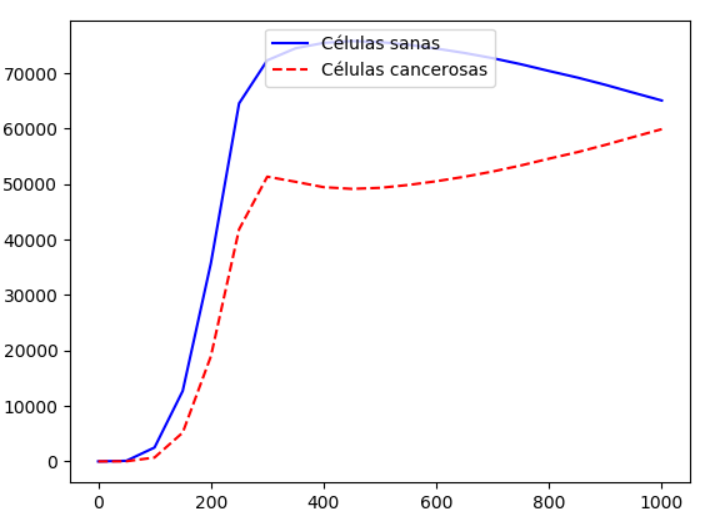
\includegraphics[scale=0.8]{figures/experiments/exp3/healthvscarcino}
\caption{Completar.}
\end{figure}

Lorem ipsum dolor sit amet, consectetur adipisicing elit, sed do eiusmod tempor incididunt ut labore et dolore magna aliqua.
Ut enim ad minim veniam, quis nostrud exercitation ullamco laboris nisi ut aliquip ex ea commodo consequat.
Duis aute irure dolor in reprehenderit in voluptate velit esse cillum dolore eu fugiat nulla pariatur.
Excepteur sint occaecat cupidatat non proident, sunt in culpa qui officia deserunt mollit anim id est laborum.

\begin{figure}[h]
\centering
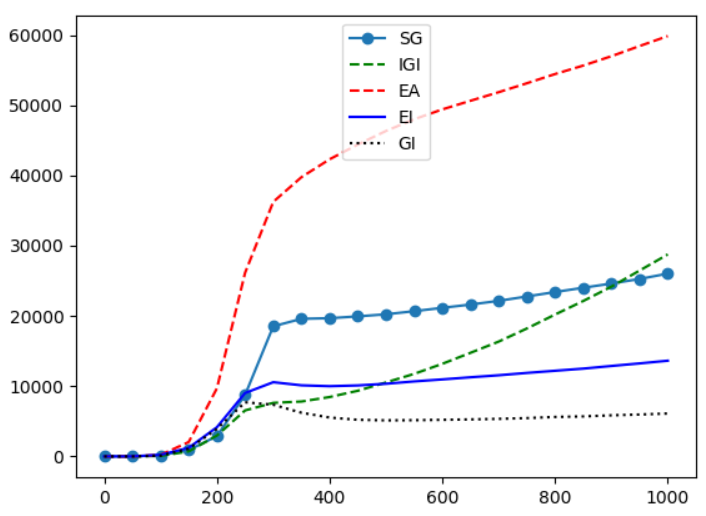
\includegraphics[scale=0.8]{figures/experiments/exp3/mutations}
\caption{Completar.}
\end{figure}

Lorem ipsum dolor sit amet, consectetur adipisicing elit, sed do eiusmod tempor incididunt ut labore et dolore magna aliqua.
Ut enim ad minim veniam, quis nostrud exercitation ullamco laboris nisi ut aliquip ex ea commodo consequat.
Duis aute irure dolor in reprehenderit in voluptate velit esse cillum dolore eu fugiat nulla pariatur.
Excepteur sint occaecat cupidatat non proident, sunt in culpa qui officia deserunt mollit anim id est laborum.

\begin{figure}[h]
\centering
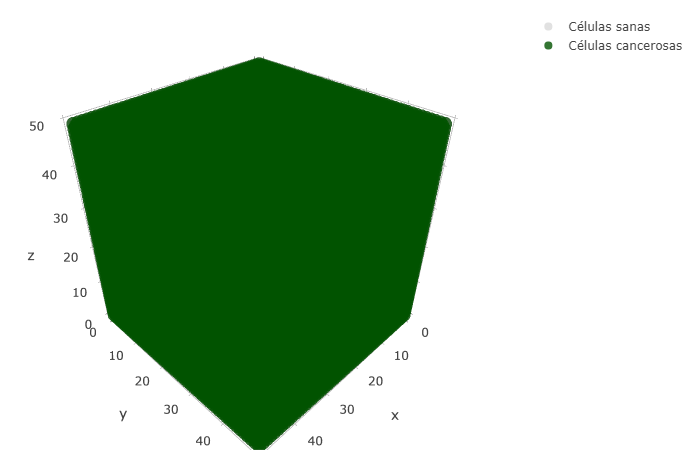
\includegraphics[scale=0.6]{figures/experiments/exp3/grid}
\caption{Completar.}
\end{figure}

Lorem ipsum dolor sit amet, consectetur adipisicing elit, sed do eiusmod tempor incididunt ut labore et dolore magna aliqua.
Ut enim ad minim veniam, quis nostrud exercitation ullamco laboris nisi ut aliquip ex ea commodo consequat.
Duis aute irure dolor in reprehenderit in voluptate velit esse cillum dolore eu fugiat nulla pariatur.
Excepteur sint occaecat cupidatat non proident, sunt in culpa qui officia deserunt mollit anim id est laborum.


    \chapter{Conclusión}
    Lorem ipsum dolor sit amet, consectetur adipisicing elit, sed do eiusmod tempor incididunt ut labore et dolore magna aliqua.
Ut enim ad minim veniam, quis nostrud exercitation ullamco laboris nisi ut aliquip ex ea commodo consequat.
Duis aute irure dolor in reprehenderit in voluptate velit esse cillum dolore eu fugiat nulla pariatur.
Excepteur sint occaecat cupidatat non proident, sunt in culpa qui officia deserunt mollit anim id est laborum.


    \chapter*{Glosario de términos}
    \begin{description}
    \item[\textbf{Adenoma}] Masa anormal que tiene un comportamiento benigno, es decir, un crecimiento leve y una invasividad de tejido adyacente bajo.
    \item[\textbf{ADN}] Abreviación de ácido desoxirribonucleico, consiste en un ácido nucléico que contiene las instrucciones genéticas usadas en el desarrollos y funcionamiento de todos los organismos vivos.
    \item[\textbf{Apoptosis}] Mecanismo de muerte celular programada para controlar y frenar el crecimiento de células que tienen su código genético dañado y, en consecuencia, pueden provocar problemas en el organismo.
    \item[\textbf{Cáncer}] Nombre genérico para describir a las enfermedades que causa proliferación descontrolada de células que provocan la aparición de masas anormales.
    \item[\textbf{Carcinoma}] Masa anormal que tiene un comportmaiento maligno, es decir, tiene una tasa de crecimiento e invasividad alta.
    \item[\textbf{Genoma}] Conjunto de genes contenidos en el cromosomas.
    \item[\textbf{Mitosis}] Proceso de reproducción de una célula, mediante el cual, se crea una copia exacta de la misma. Puede contener daños genéticos que no se dan en la célula original.
    \item[\textbf{Singleton}] Lorem ipsum dolor sit amet, consectetur adipisicing elit, sed do eiusmod tempor incididunt ut labore et dolore magna aliqua.
    \item[\textbf{Telómero}] Lorem ipsum dolor sit amet, consectetur adipisicing elit, sed do eiusmod tempor incididunt ut labore et dolore magna aliqua.
\end{description}


    \printbibliography

\end{document}
